\section{Web Service的发布和查询}

\subsection{在注册表中发布 Web Service}
Web服务的实现部署在可通过互联网访问的应用服务器上,然后发布到互联网上的服务注册表中,以便任何用户都可以找到它。

服务注册表提供服务请求者需要发现服务提供者及其Web服务的信息,而不是实际的实现
\vspace{-0.8em}
\begin{multicols}{3}
    \begin{itemize}
        \item 服务名称
        \item 服务提供者的名称
        \item 服务的WSDL文件的URL
    \end{itemize}
\end{multicols}
\vspace{-1em}

Web Services发布方法
\begin{itemize}
    \item 发布到一个集中的服务注册表:UDDI
    \item 发布到一个分布式的服务注册表:Web服务检查语言(WS-Inspection Language, WSIL)
\end{itemize}

\begin{figure}[H]
    \vspace{-0.5em}
	\centering
	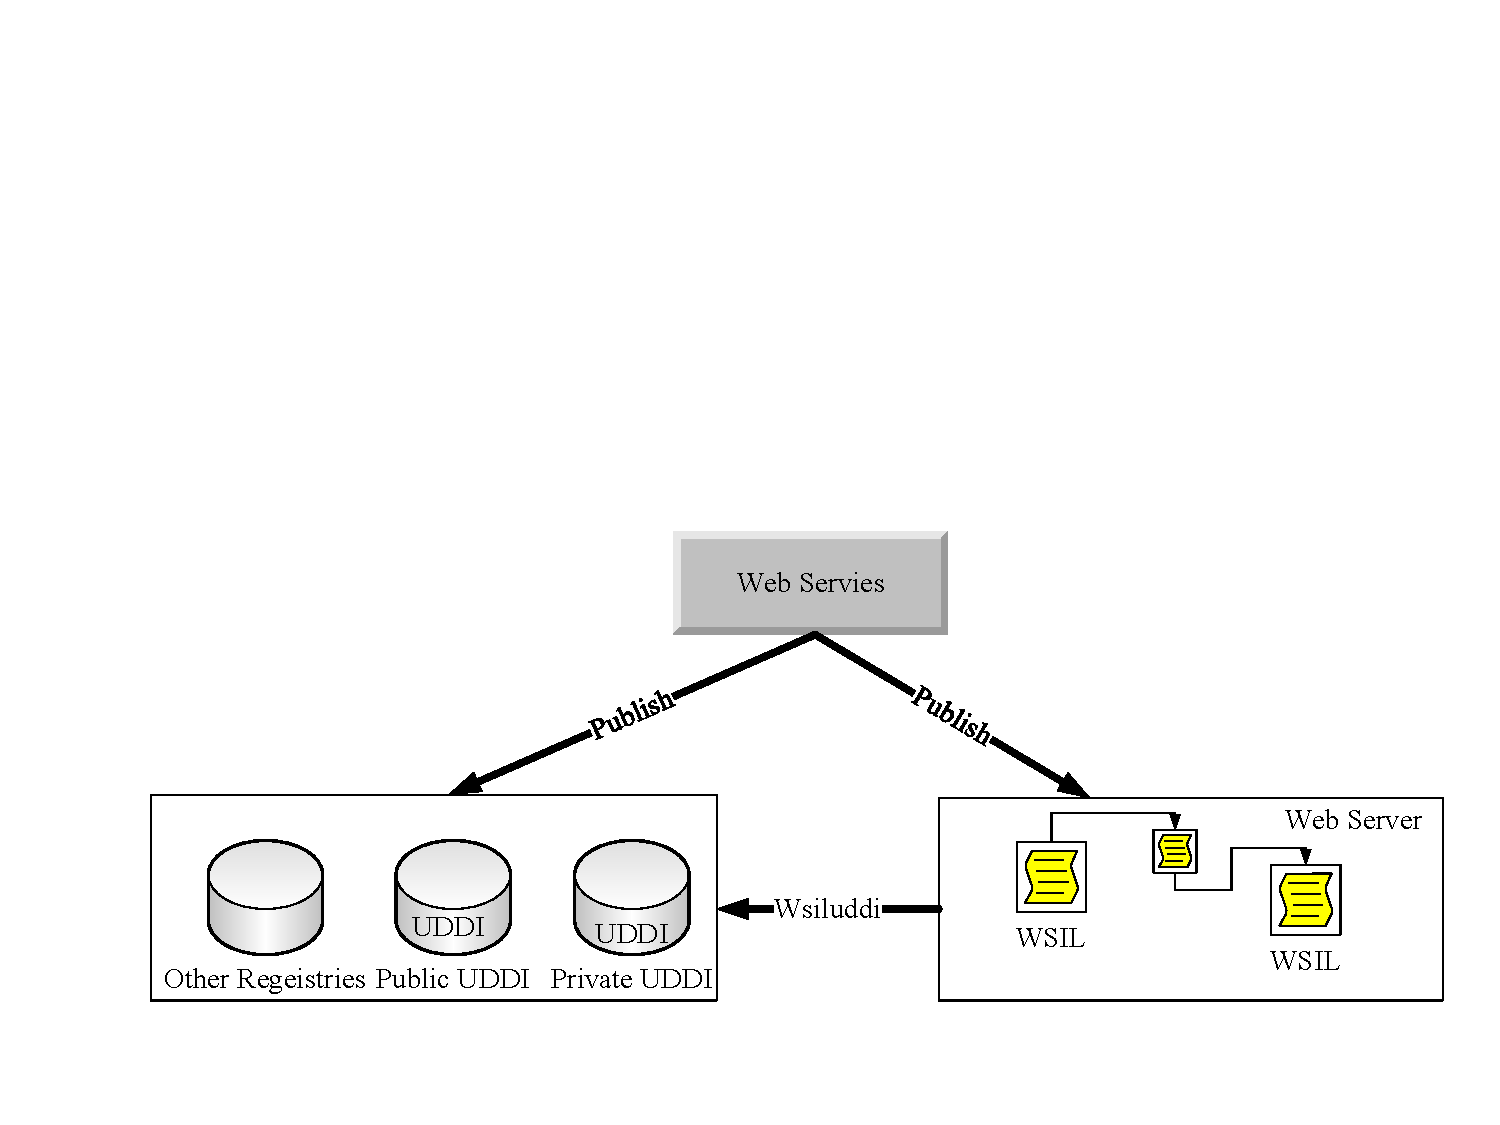
\includegraphics[width=0.7\textwidth]{images/Web services publishing approaches.pdf}
    \vspace{-1em}
\end{figure}

\subsection{UDDI}

\subsubsection{UDDI的作用}
UDDI(Universal Description, Discovery, and Integration)被用来提供发布和查找 Web Service 的元服务。它可以用来针对丰富的元信息进行查找

UDDI 采用 XML 格式,来存放注册 Web Service 的描述性息,主要提供以下信息:
\vspace{-0.8em}
\begin{multicols}{2}
    \begin{itemize}
        \item WHO :业务的基本信息(谁提供服务)
        \item WHAT :分类信息(服务完成哪些功能)
        \item WHERE :注册信息(哪里完成服务的调用)
        \item HOW :关于服务接口的注册引用及其它属性(采用什么方式访问)
    \end{itemize}
\end{multicols}
\vspace{-1em}

UDDI 使用注册实体记录 Web Service 的发布信息,注册实体可分为三类:
\begin{itemize}
    \item 白页:关于名称、地址、具体联系方式等基本信息
    \item 黄页:针对业务或服务进行分类的信息
    \vspace{-0.8em}
    \begin{multicols}{3}
        \begin{itemize}
        \item 按行业:NAICS
        \item 按产品/服务:UNSPSC
        \item 按位置:ISO地理分类标准
        \end{itemize}
    \end{multicols}
    \vspace{-1em}
    \item 绿页:服务中的技术性信息,对于有关技术信息进行解耦
\end{itemize}

\subsubsection{UDDI结构}
UDDI包括五个主要元素,并使用XML Schema来正式表达其数据结构
\vspace{-0.8em}
\begin{multicols}{2}
    \begin{itemize}
        \item businessEntity:商业实体信息及其提供的服务
        \item businessService:商业实体所提供的服务
        \item bindingTemplates:如何调用一个服务
        \item tModel (Technical Models):特定概念和结构(主要是对于绿页的抽象)
        \item publisherAssertion:表达商业关系
    \end{itemize}
\end{multicols}
\vspace{-1em}

\paragraph*{businessEntity:商业实体信息及其提供的服务}~{} \par
\begin{figure}[H]
    \vspace{-0.5em}
	\centering
	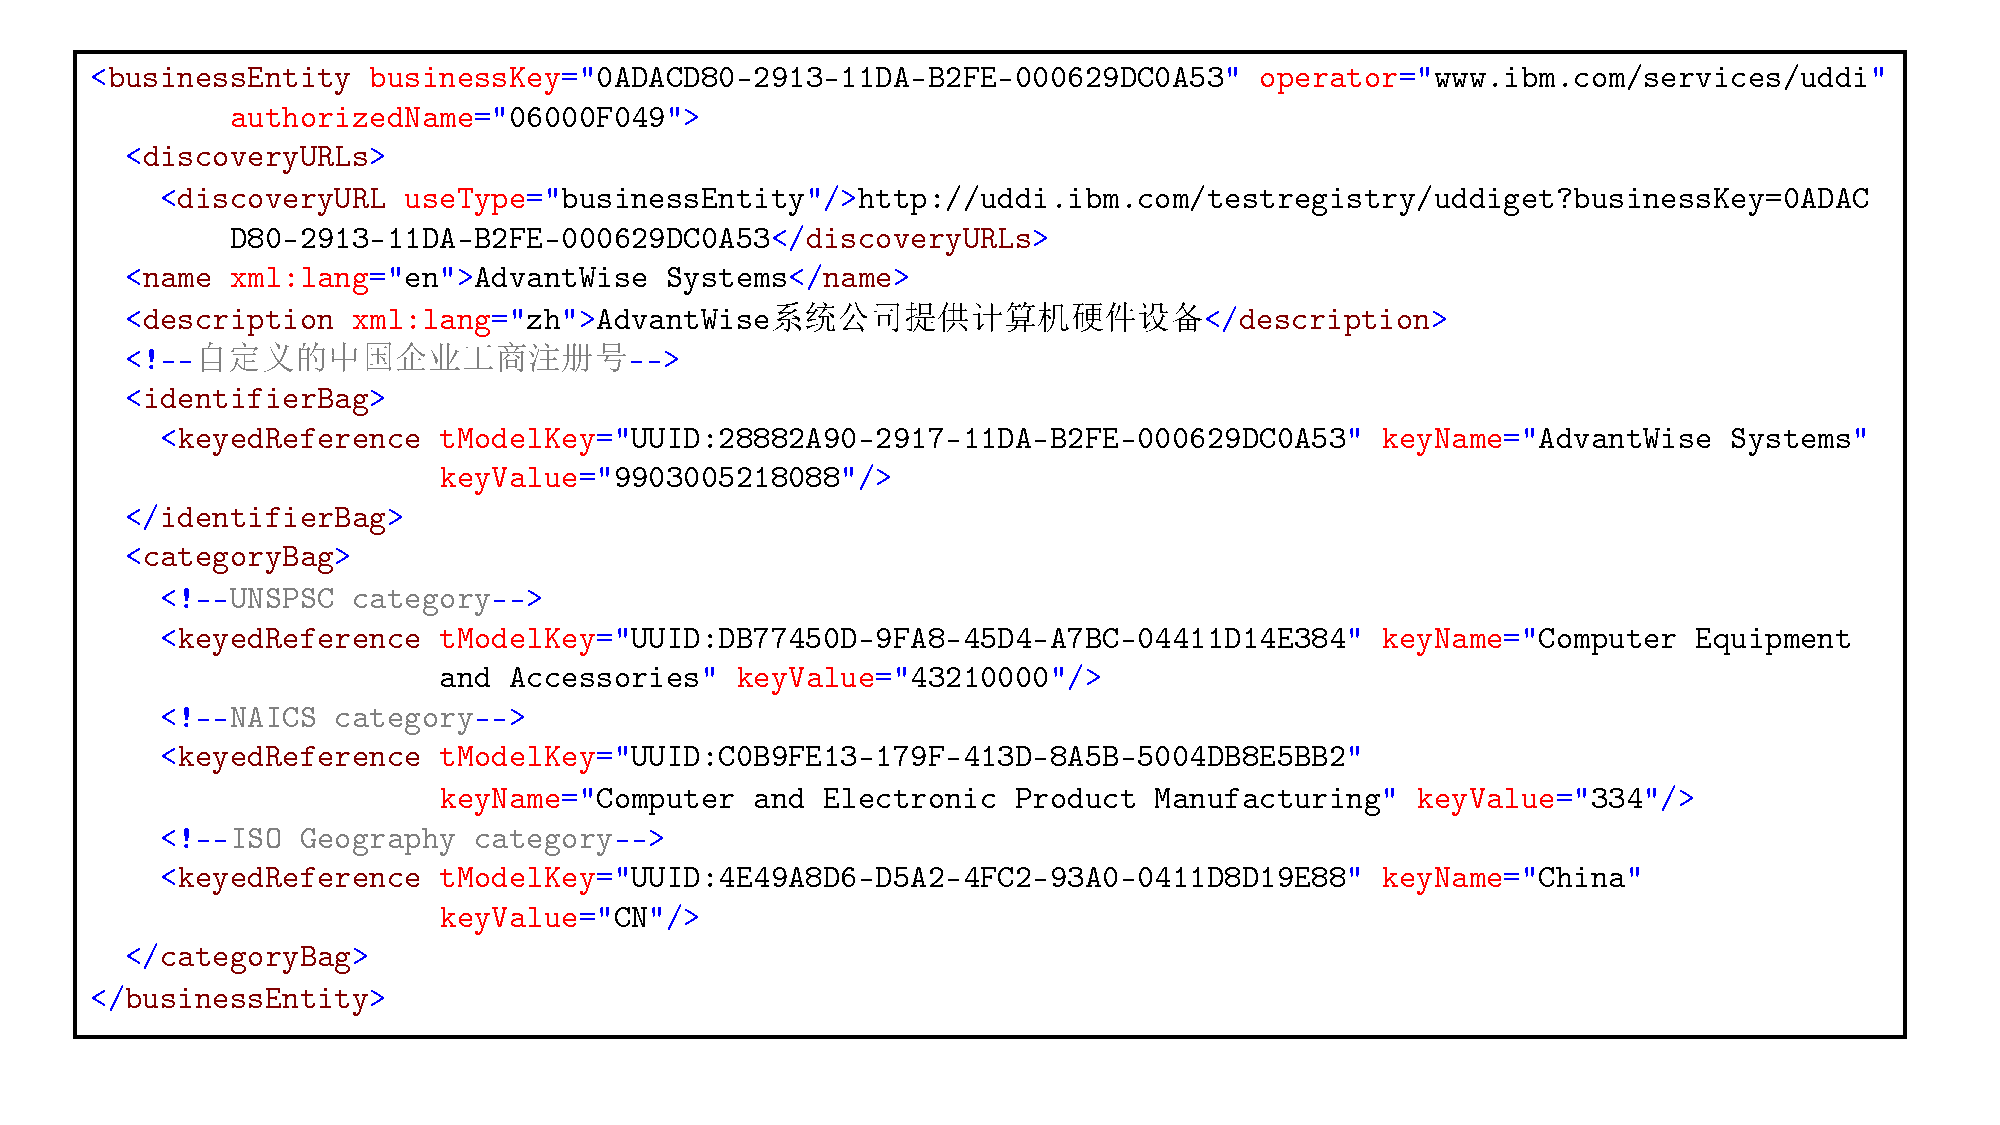
\includegraphics[width=\textwidth]{images/businessEntitiy.pdf}
    \vspace{-3em}
\end{figure}

\paragraph*{businessService:商业实体所提供的服务}~{} \par
\begin{figure}[H]
    \vspace{-0.5em}
	\centering
	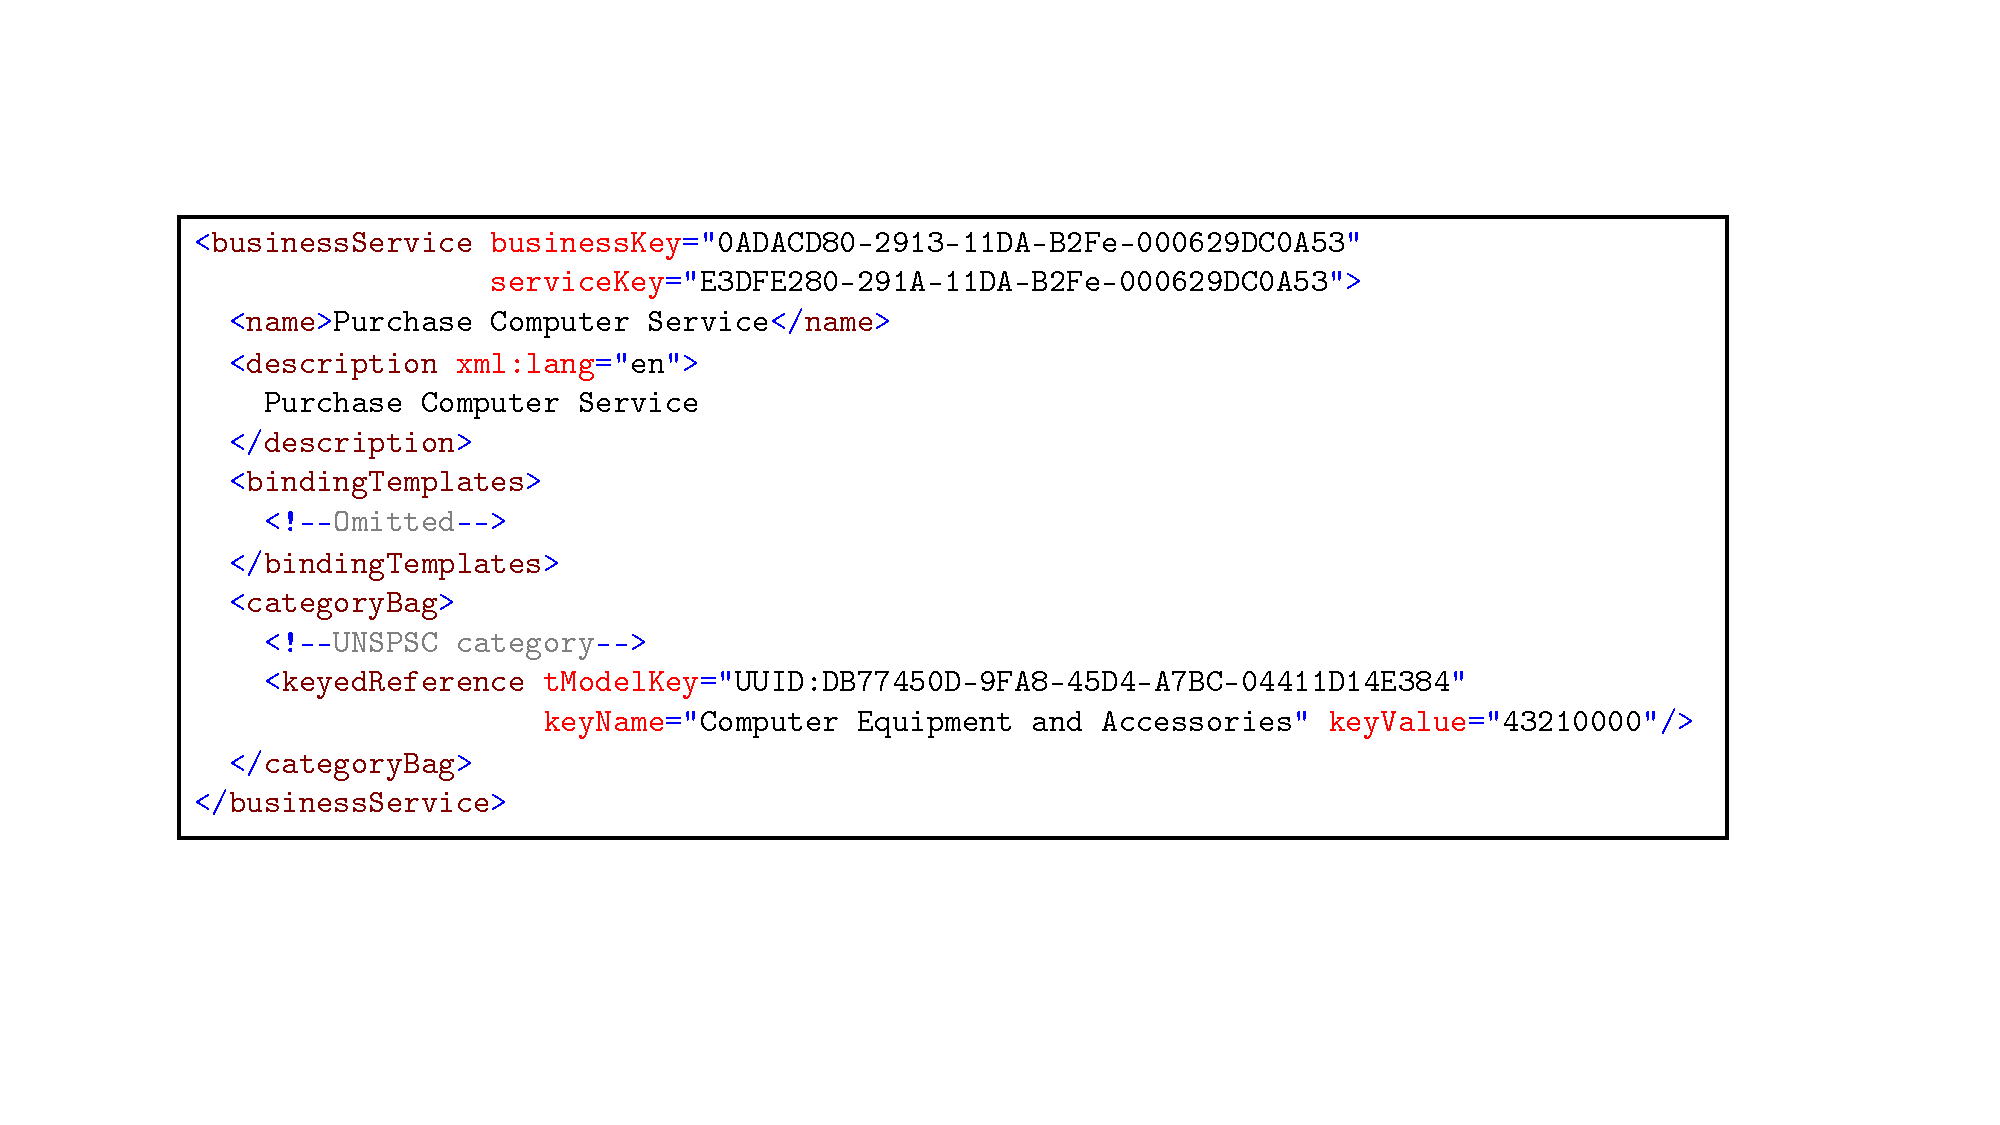
\includegraphics[width=0.9\textwidth]{images/businessService.pdf}
    \vspace{-1em}
\end{figure}

\paragraph*{bindingTemplates:如何调用一个服务}~{} \par
\begin{figure}[H]
    \vspace{-0.5em}
	\centering
	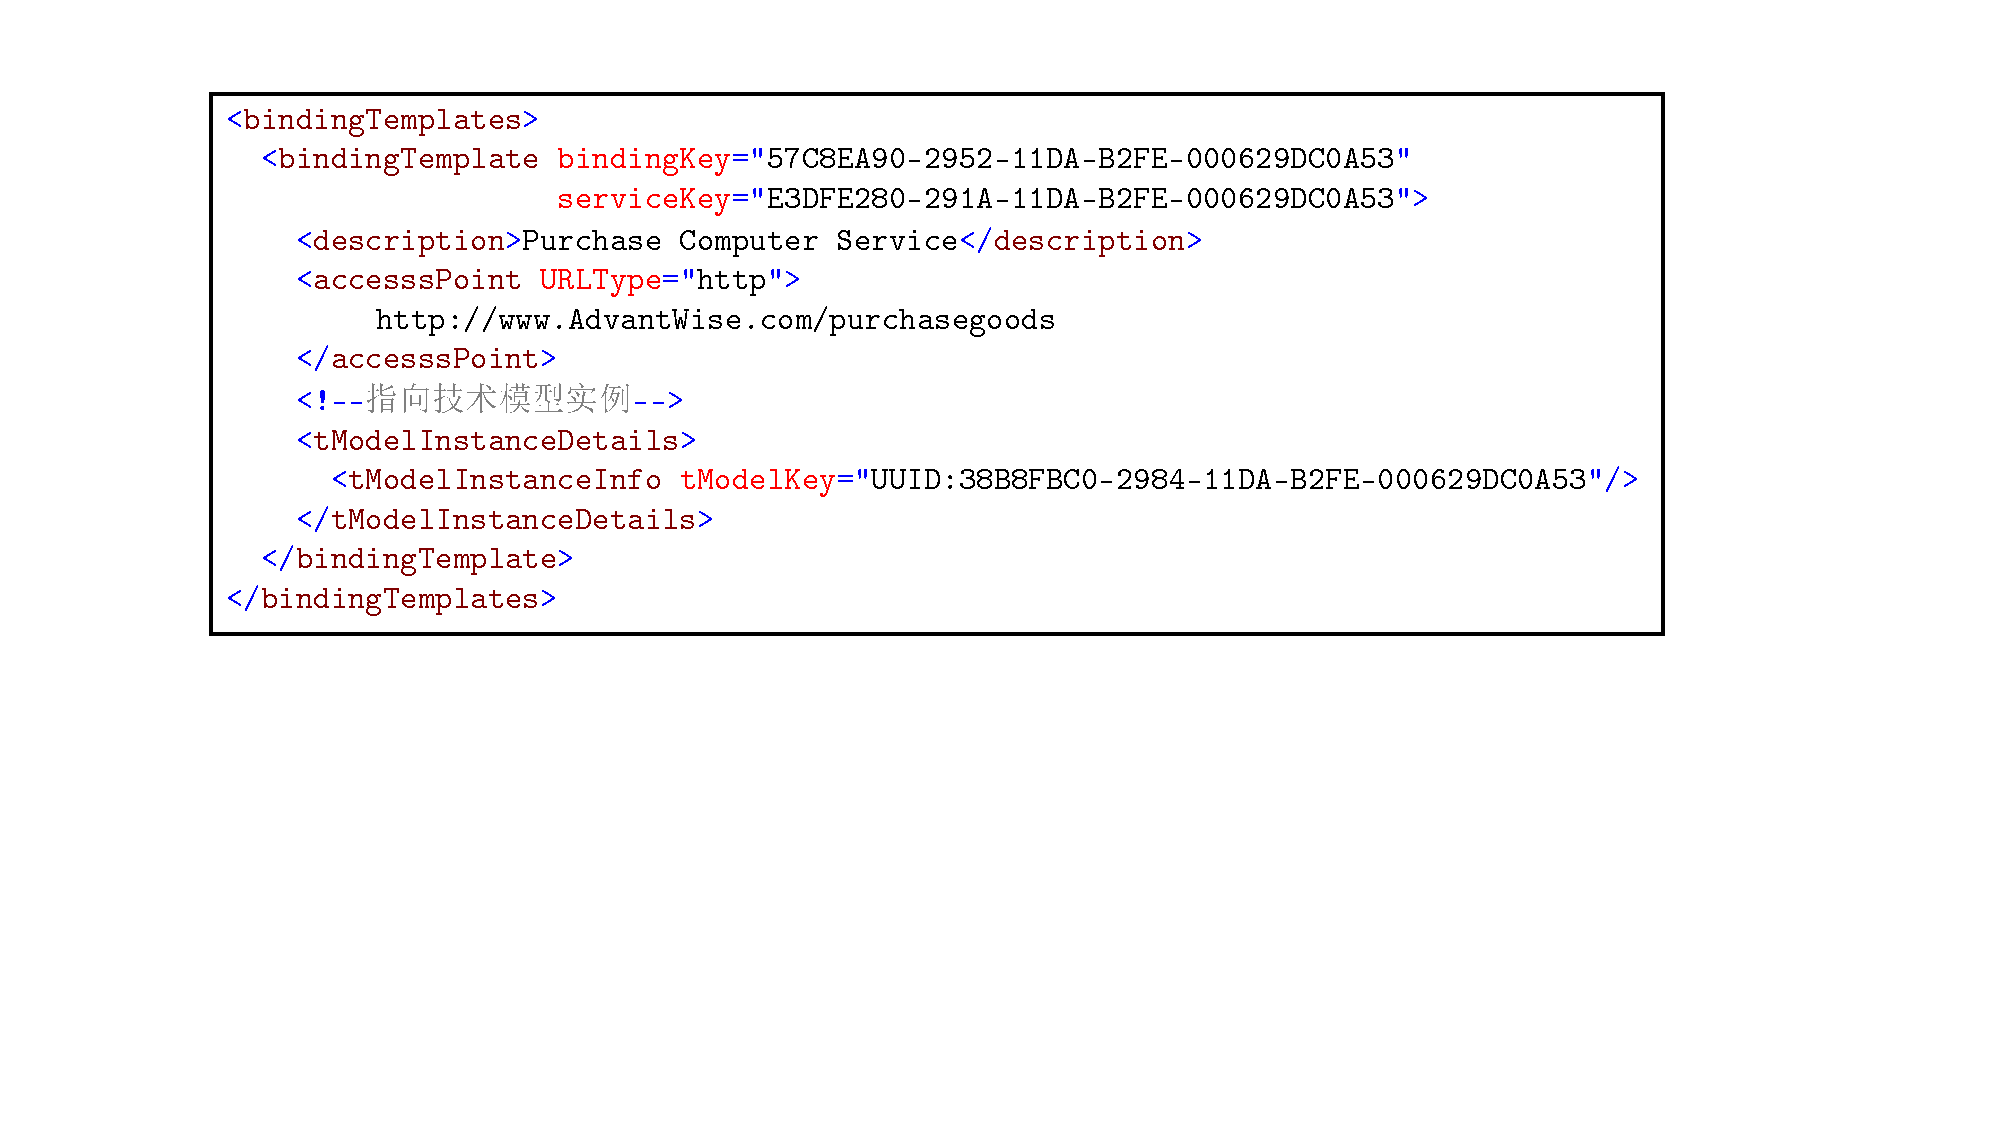
\includegraphics[width=0.9\textwidth]{images/bindingTemplates.pdf}
    \vspace{-1em}
\end{figure}

\paragraph*{tModel (Technical Models):特定概念和结构(主要是对于绿页的抽象)}~{} \par
\begin{figure}[H]
    \vspace{-0.5em}
	\centering
	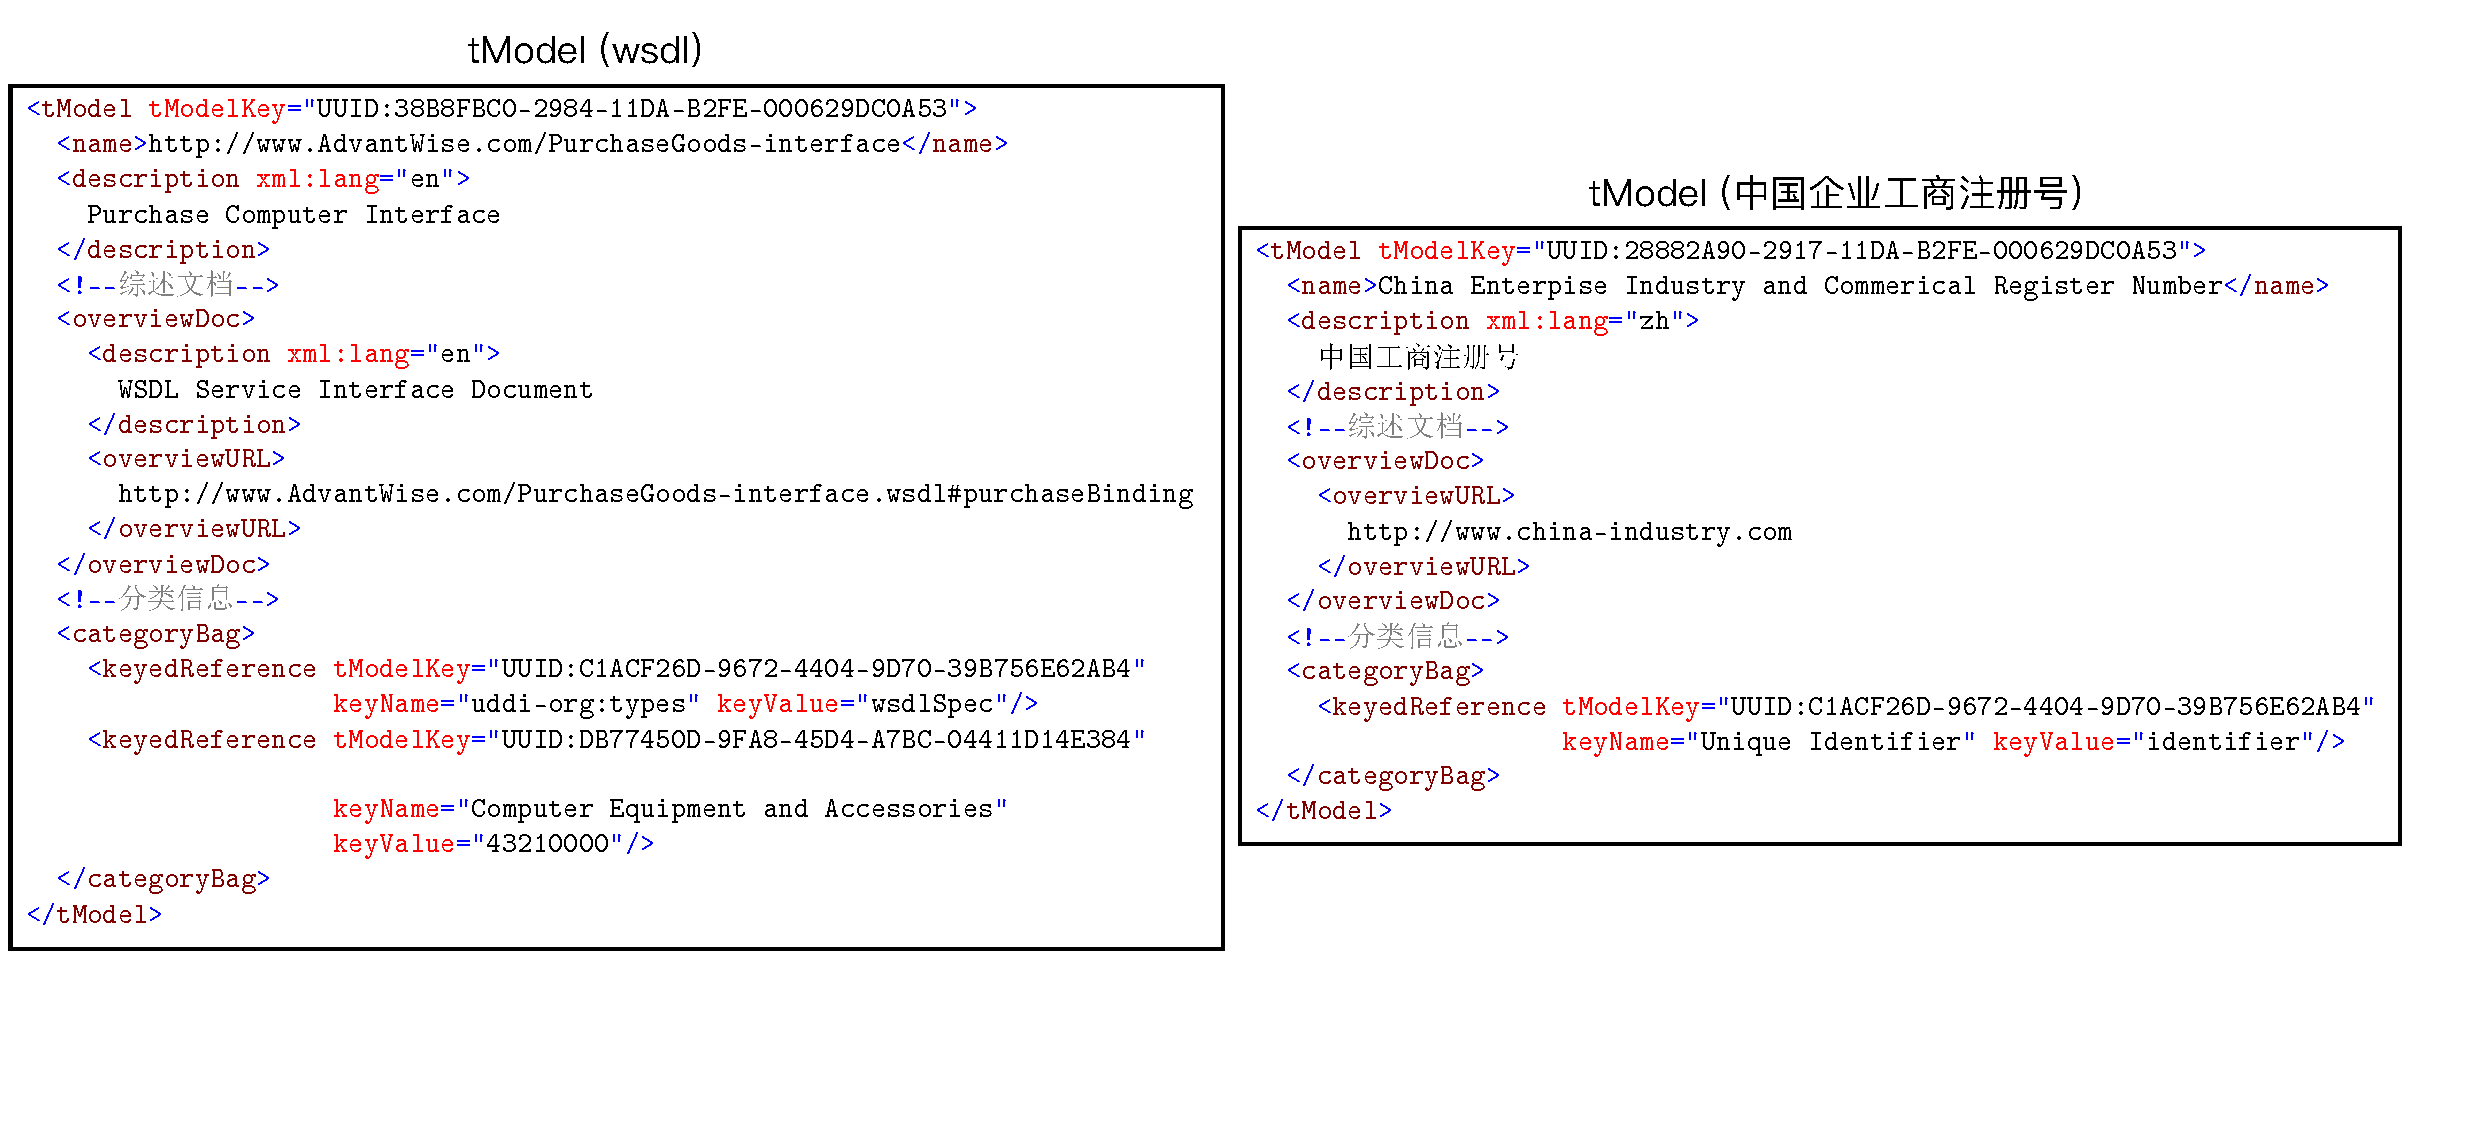
\includegraphics[width=\textwidth]{images/tModel.pdf}
    \vspace{-3em}
\end{figure}

\paragraph*{publisherAssertion:表达商业关系}~{} \par
\begin{figure}[H]
    \vspace{-0.5em}
	\centering
	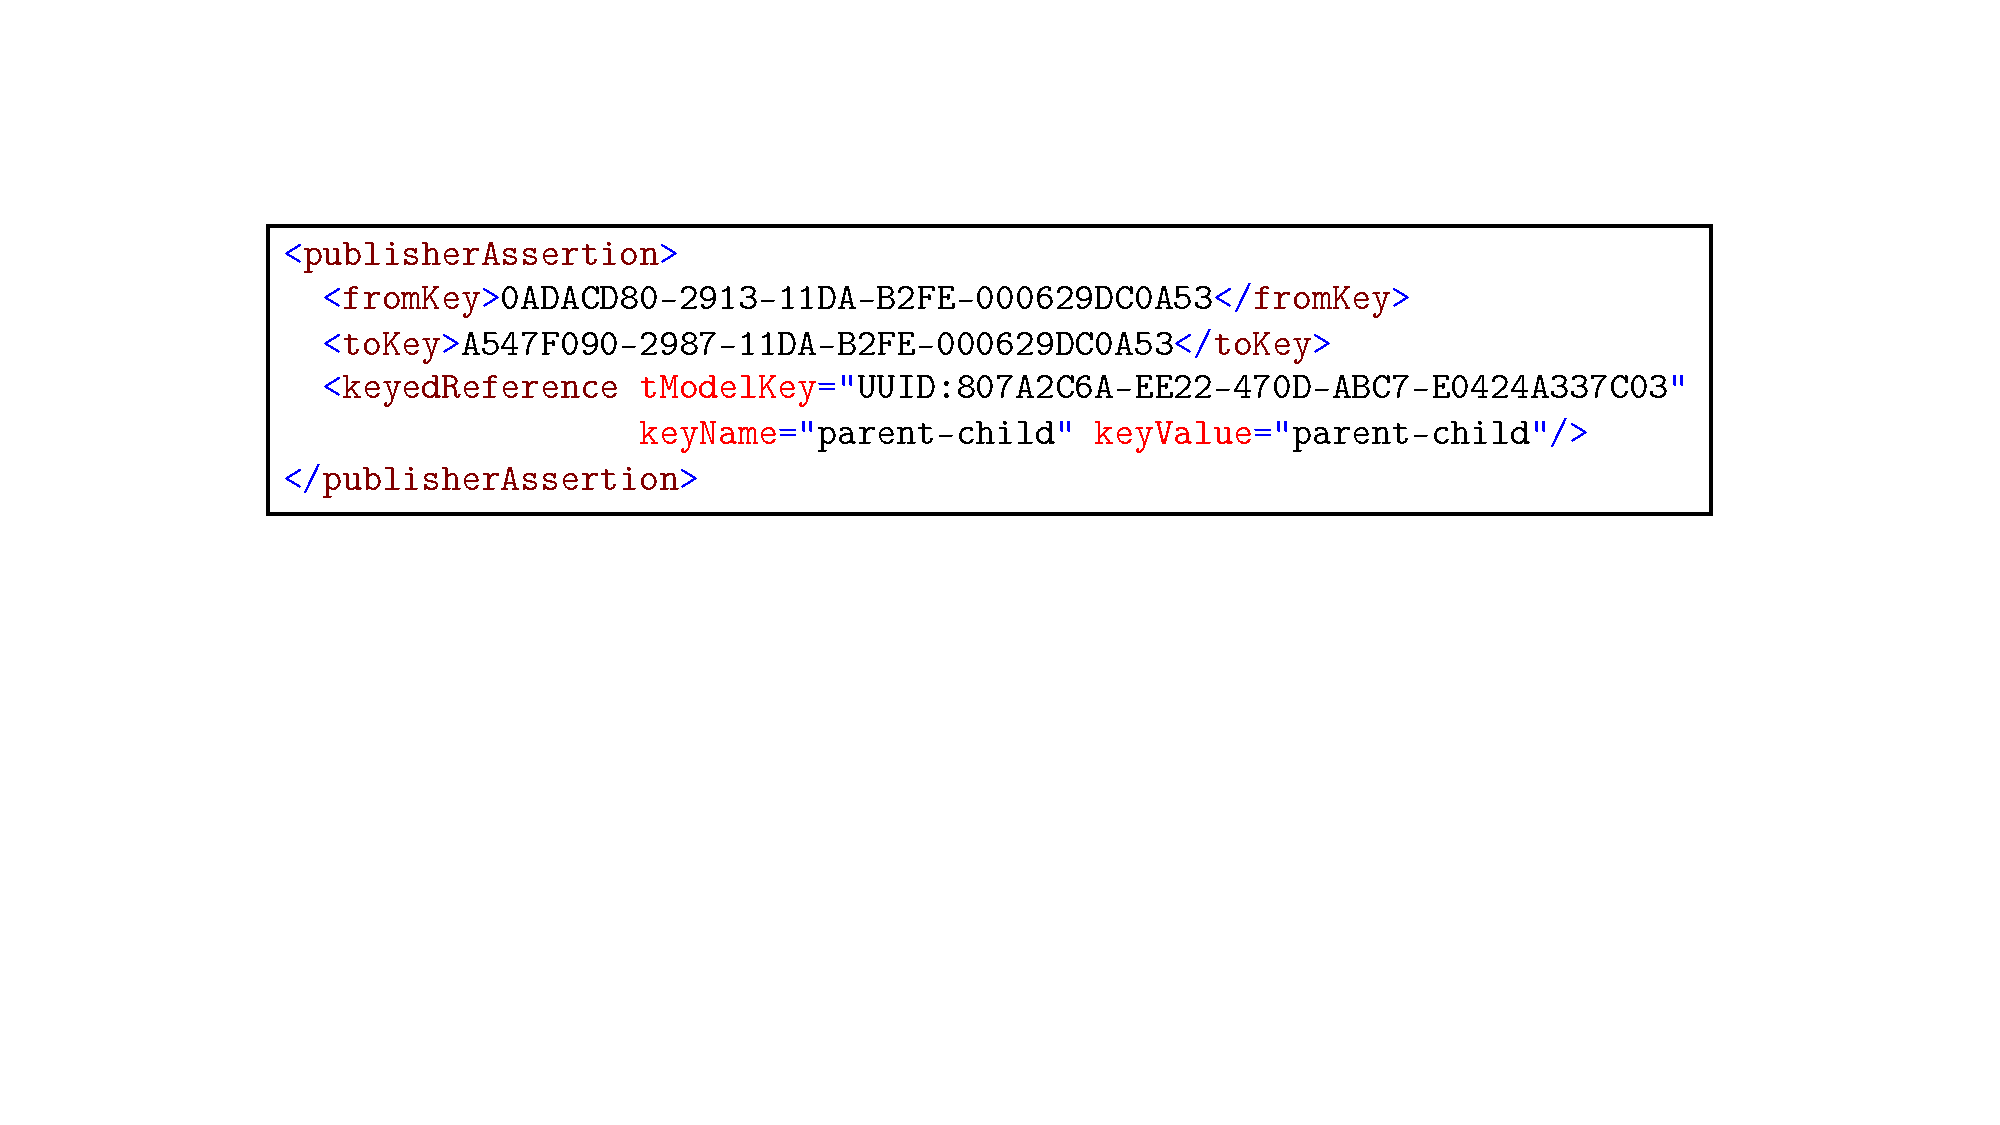
\includegraphics[width=0.75\textwidth]{images/publisherAssertion.pdf}
    \vspace{-1em}
\end{figure}

\paragraph*{UDDI元素间关系与基本类型系统}~{} \par
\begin{figure}[H]
	\setcounter{subfigure}{0}
	\centering
	\vspace{-0.5em}	
	\subfloat[UDDI元素间关系]{
	\begin{minipage}[t]{0.47\linewidth}
	\centering
	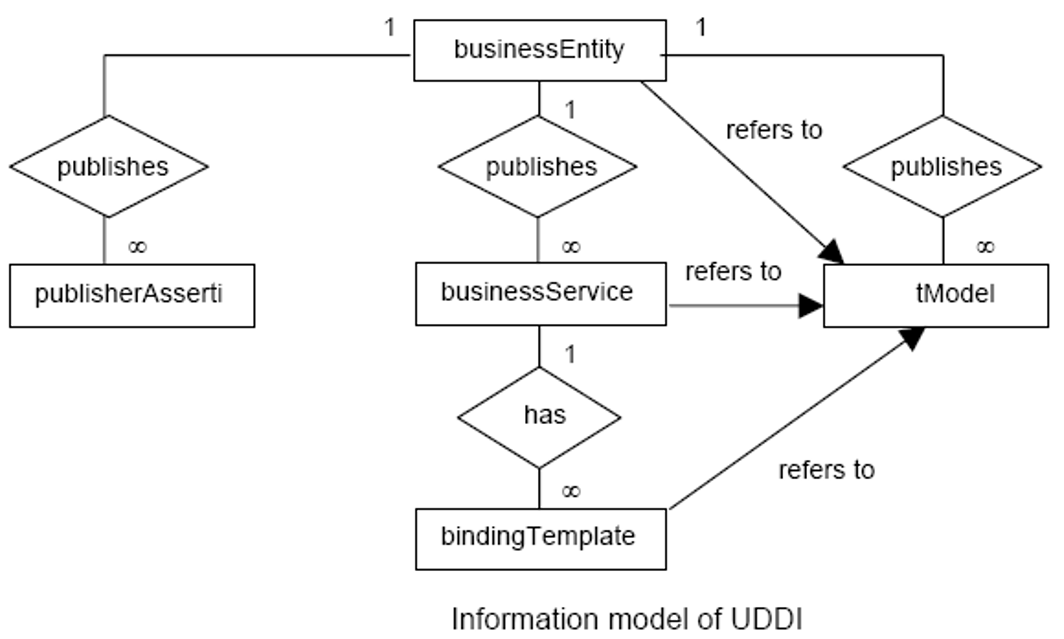
\includegraphics[width=\linewidth]{images/UDDI元素间关系.png}
	\end{minipage}
	}
	\subfloat[UDDI基本类型系统]{
	\begin{minipage}[t]{0.47\linewidth}
	\centering
	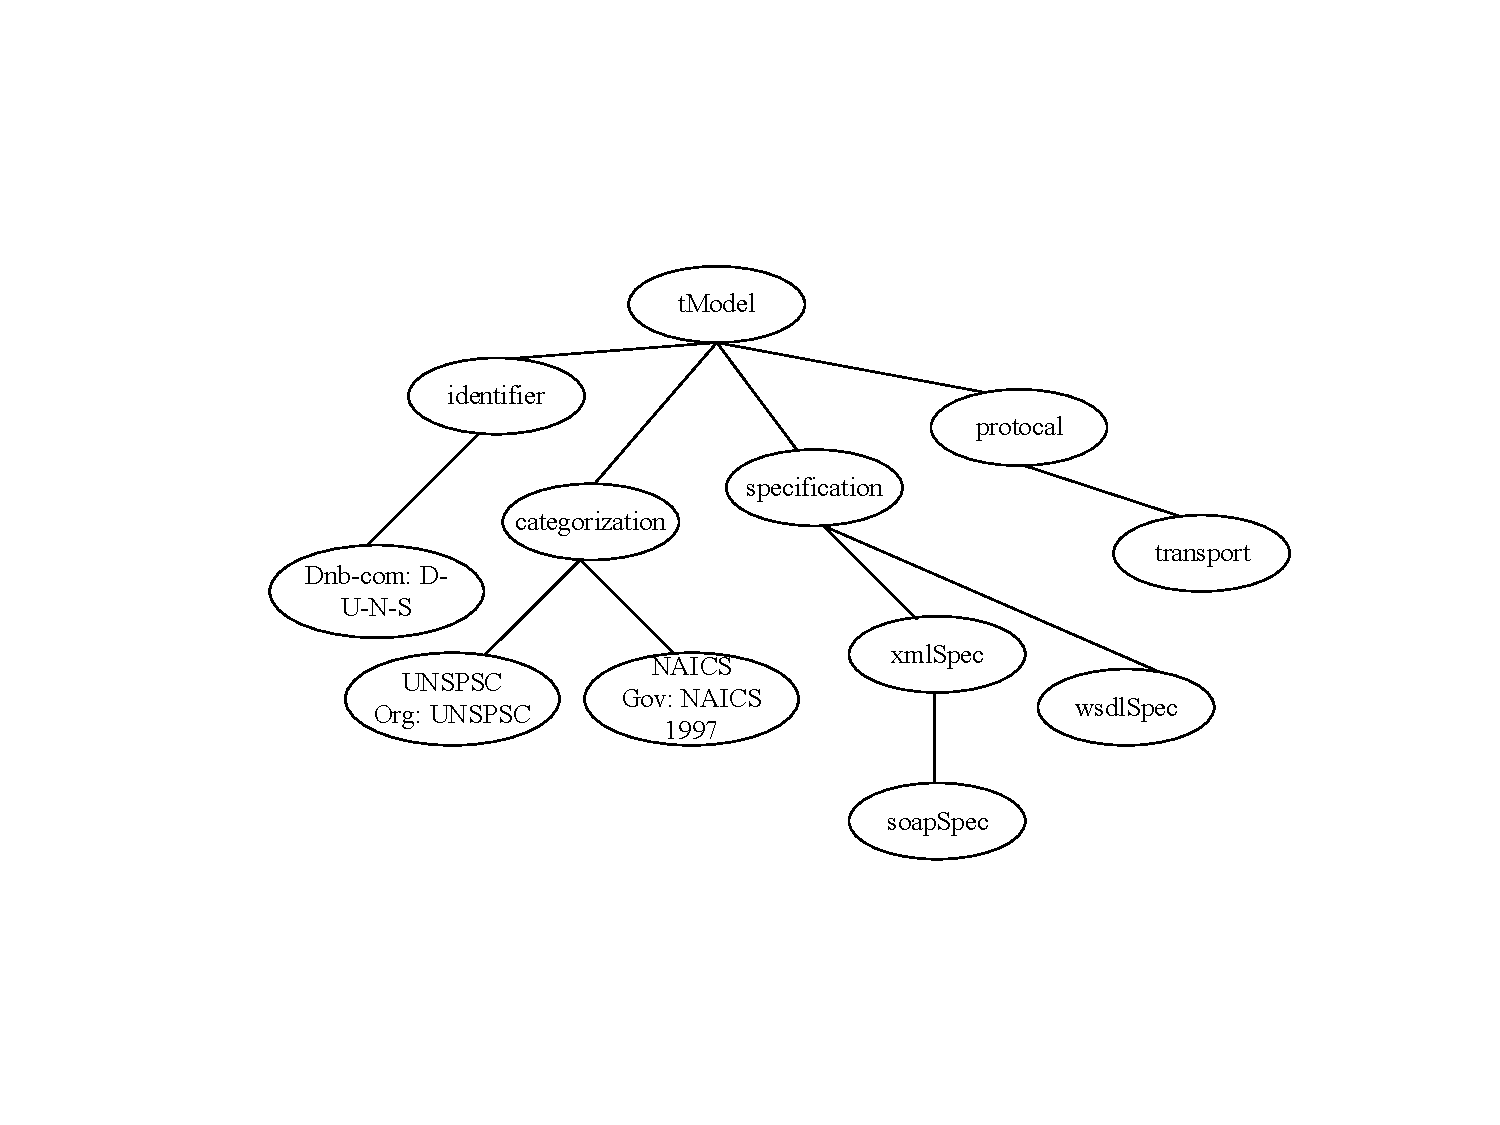
\includegraphics[width=\linewidth]{images/UDDI Basic Type System.pdf}
	\end{minipage}
	}
	\centering
	\vspace{-1em}
\end{figure}

\subsubsection{WSDL与UDDI间的映射}
\begin{figure}[H]
    \vspace{-0.5em}
	\centering
	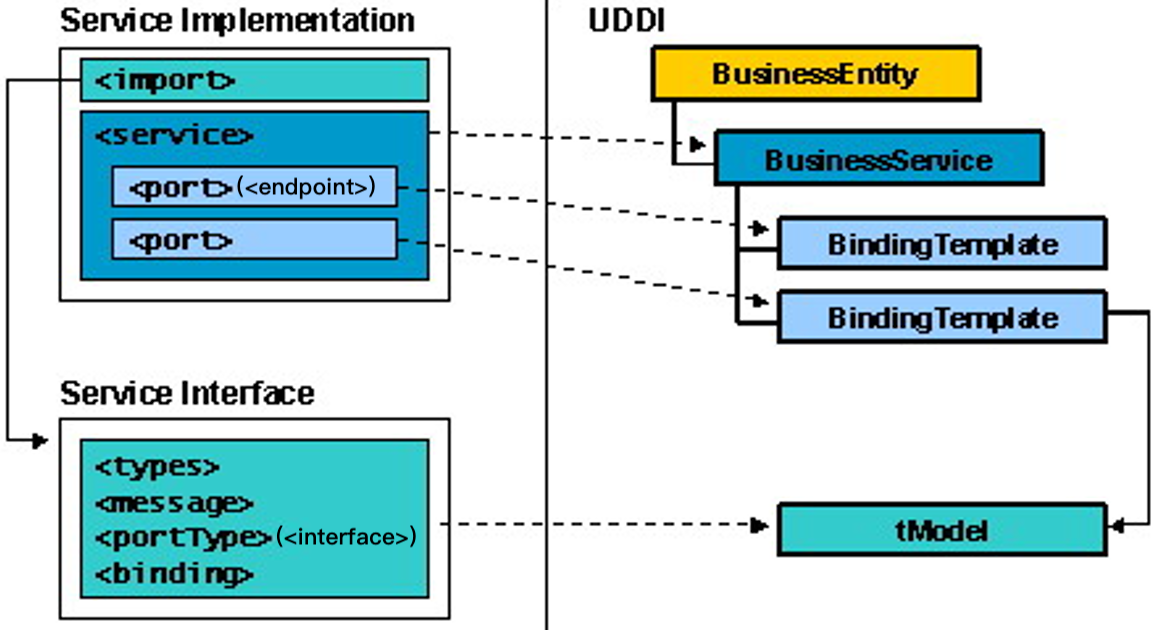
\includegraphics[width=0.65\textwidth]{images/Mapping from WSDL to UDDI.png}
    \vspace{-1em}
\end{figure}

将WSDL绑定到UDDI
\begin{figure}[H]
    \vspace{-0.5em}
	\centering
	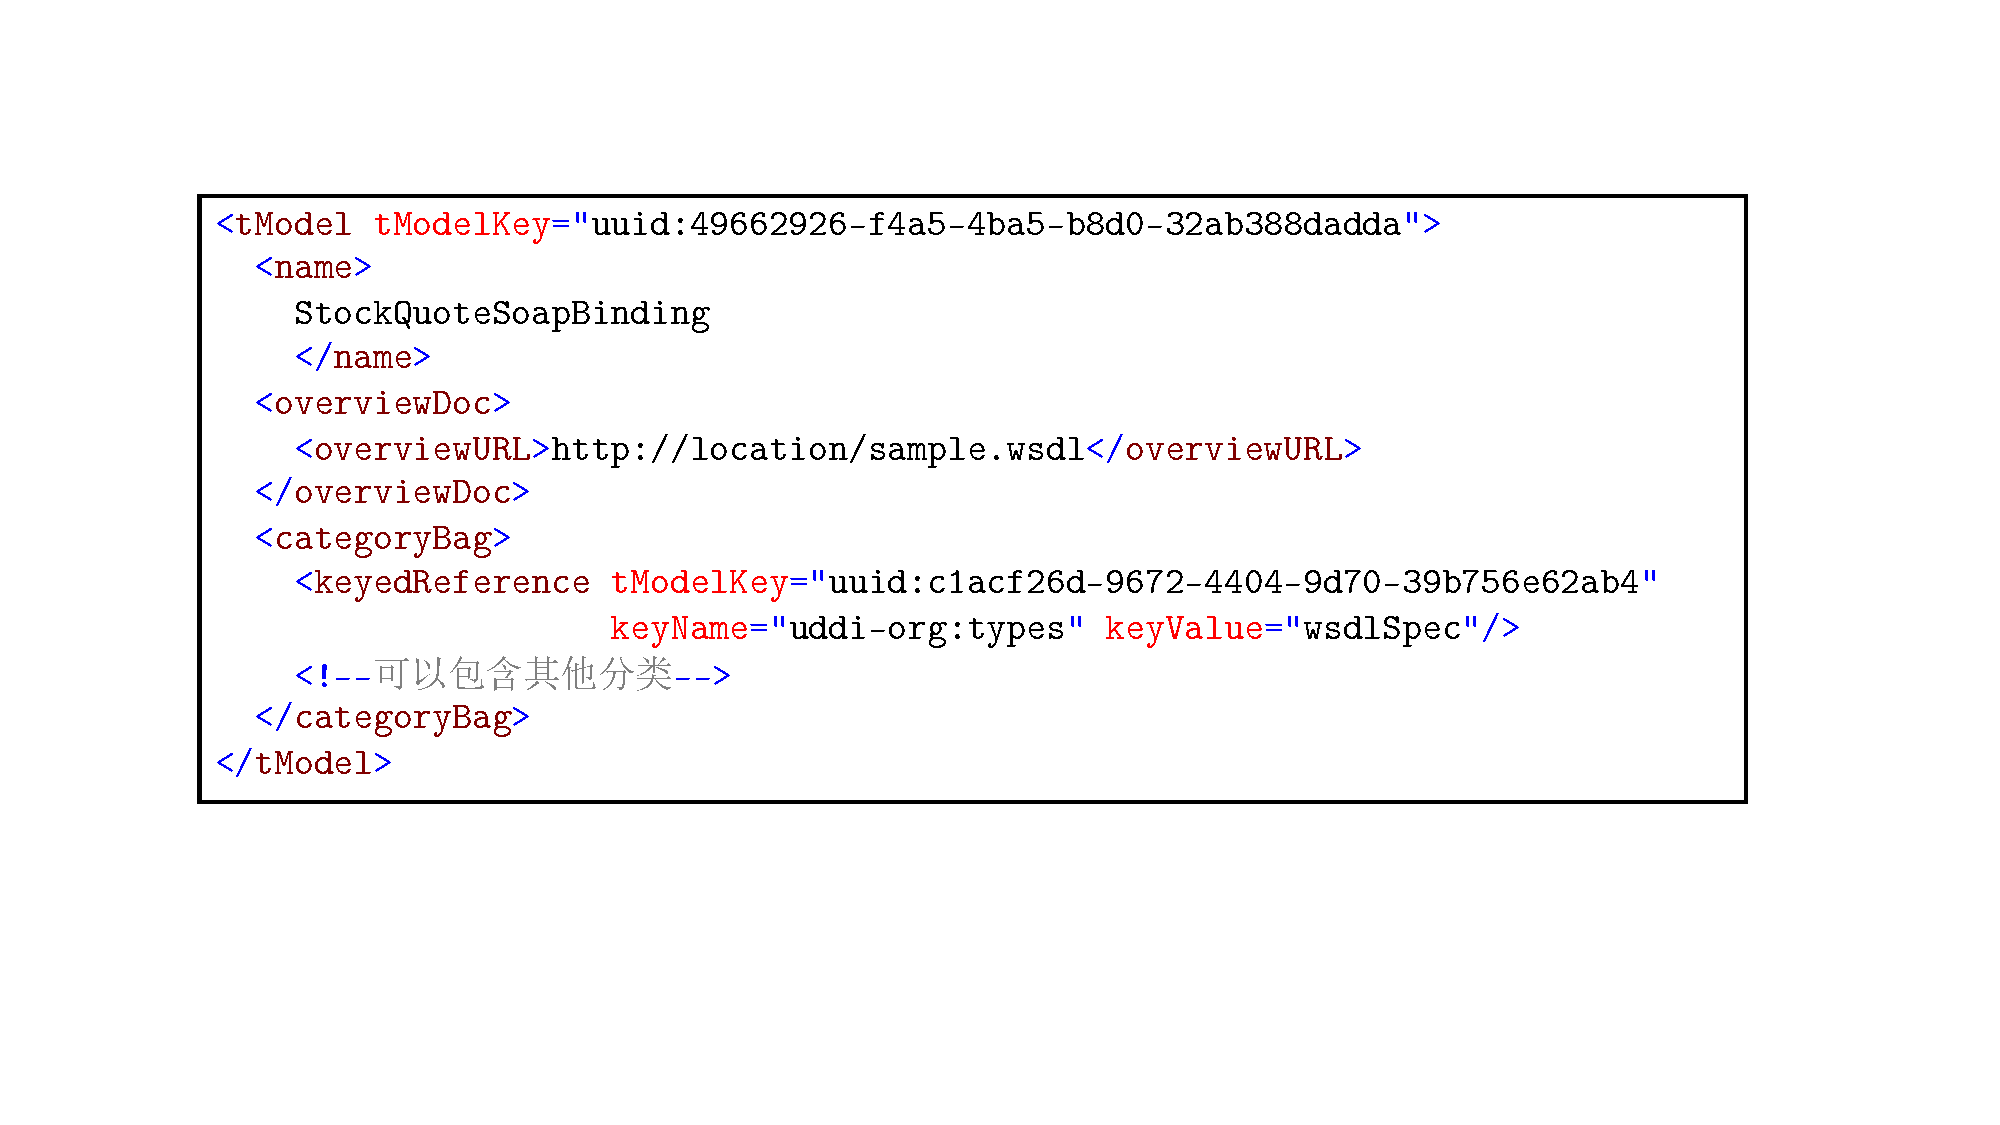
\includegraphics[width=0.75\textwidth]{images/将WSDL绑定到UDDI.pdf}
    \vspace{-1em}
\end{figure}

\subsubsection{UDDI API}
对于分类、编目和管理Web服务,UDDI注册库提供了一个标准方式,以便于能够发现和使用这些Web服务
\begin{itemize}
    \item 业务和提供者可以按标准方式使用UDDI来表示Web服务信息
    \item UDDI使用SOAP作为它的传输层
\end{itemize}

UDDI API是一个接口,可以接受封装在SOAP信封中的XML消息
\begin{itemize}
    \item 所有的UDDI交互都使用请求/响应模式
    \item 可以使用出查询API来搜索和读取UDDI注册库中的数据,并可使用发布API来添加、更新和删除UDDI注册库中的数据
\end{itemize}

\subsubsection{UDDI发布API}
通过发布接口,企业可以存储和更新包含在UDDI注册库中的信息

发布API支持4类操作
\vspace{-0.5em}
\begin{spacing}{1.2}
    \begin{longtable}{|m{1.5cm}<{\centering}|m{11.5cm}|}
    \hline
    \textbf{操作} & \multicolumn{1}{c|}{\textbf{描述}} \\ \hline
    授权 &
    客户端可以获得相应的访问权限、获取授权令牌、终止会话和授权令牌
    \begin{itemize}[leftmargin=1.5em,itemsep=-3pt]
        \item \verb|get_authtoken|:将客户端记录到注册
        \item \verb|discard_authtoken|:终止会话,并从注册库中删除客户端
    \vspace{-1.5em}
    \end{itemize}                                           
    \\ \hline
    保存 & 客户端可以在UDDI中添加或更新信息 \\ \hline
    获取 & 可以获取客户端所发布的数据结构的概要数据 \\ \hline
    删除 & 客户端可以在UDDI中删除信息 \\ \hline
\end{longtable}
\end{spacing}
\vspace{-1.2em}

\subsection{WSIL}

\subsubsection{WSIL发布}
Web服务以XML文档的形式发布到常规Web服务器上。WSIL用于汇总现有服务描述文档的引用,引用指针可用于连接到在UDDI注册表中发布的服务,或连接到另一个WSIL文档,因此形成了WSIL链。
\begin{itemize}
    \item WSIL链接是由一系列WSIL文档组成的,每个文档描述了一个或多个相关的Web服务。在WSIL链接中,每个WSIL文档都包含一个指向下一个文档的URL,形成一个链式结构。
    \item 当服务请求者查找Web服务时,可以通过WSIL链接遍历整个文档链,找到需要的服务提供者和相关信息。WSIL链接的结构类似于超链接,但它们的目的是将服务请求者引导到与Web服务相关的信息,而不是到Web页面。  
    \item 通常,WSIL链接的第一个文档位于某个服务注册表中,其中包含了多个服务提供者的WSIL文件的链接。服务请求者可以通过访问注册表中的WSIL链接来发现服务提供者,并获取他们的Web服务的详细信息。在每个WSIL文档中,都包含了指向下一个文档的URL,使得服务请求者可以通过WSIL链接遍历整个文档链。
\end{itemize}

\subsubsection{一个WSIL链的例子}
\begin{figure}[H]
    \vspace{-0.5em}
	\centering
	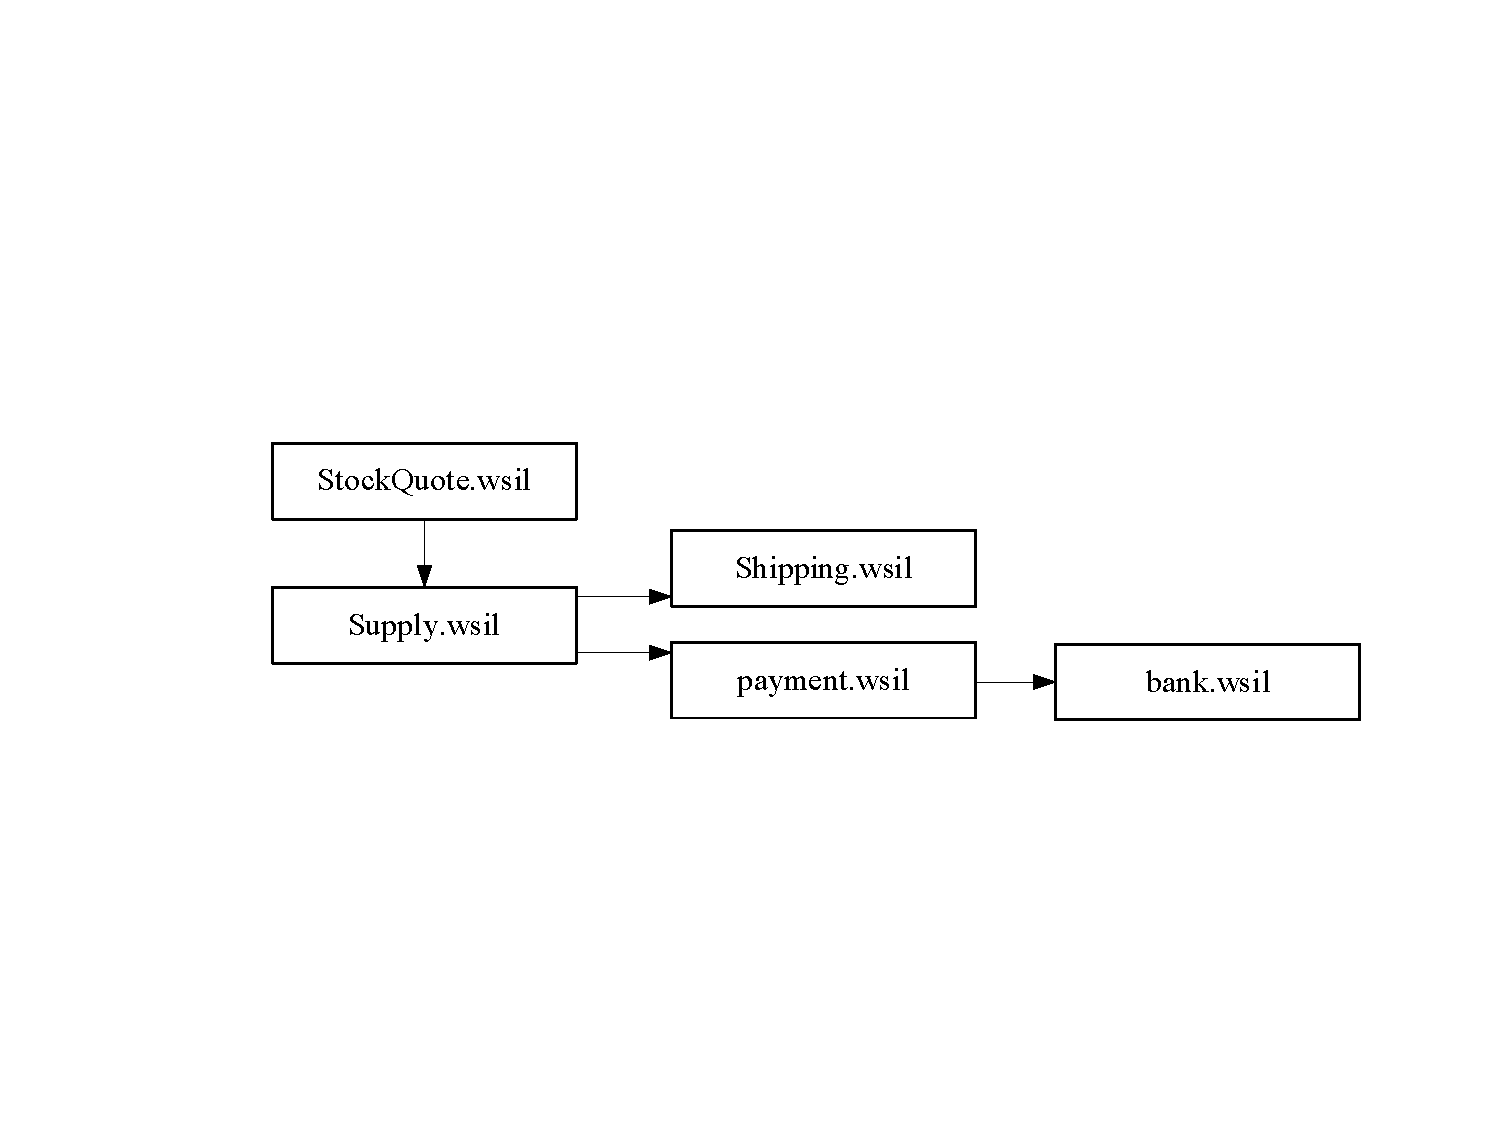
\includegraphics[width=0.6\textwidth]{images/A example of WSIL chain.pdf}
    \vspace{-1em}
\end{figure}

\paragraph*{StockQuote.wsil}~{} \par
\begin{figure}[H]
    \vspace{-0.5em}
	\centering
	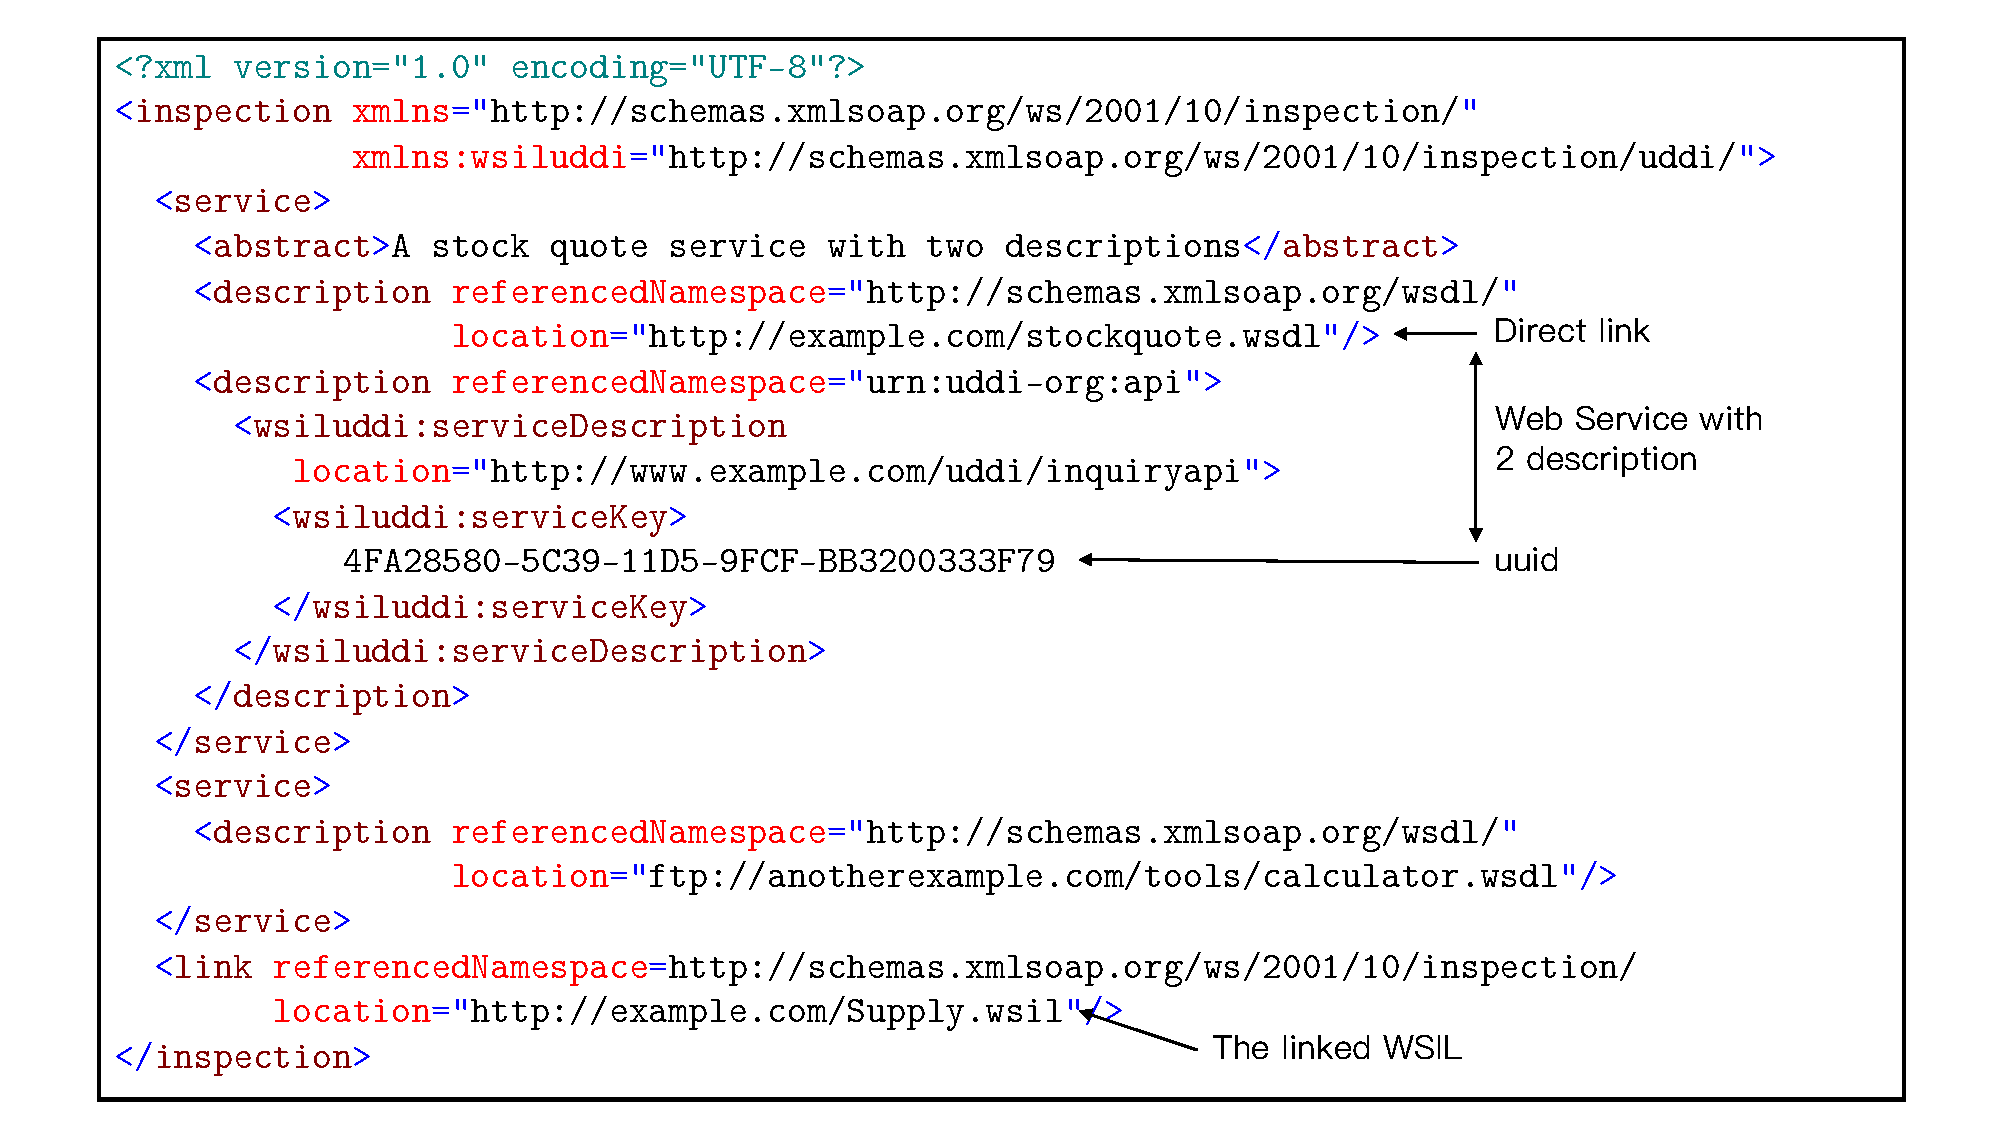
\includegraphics[width=0.8\textwidth]{images/StockQuote.wsil.pdf}
    \vspace{-1em}
\end{figure}

\paragraph*{Supply.wsil}~{} \par
\begin{figure}[H]
    \vspace{-0.5em}
	\centering
	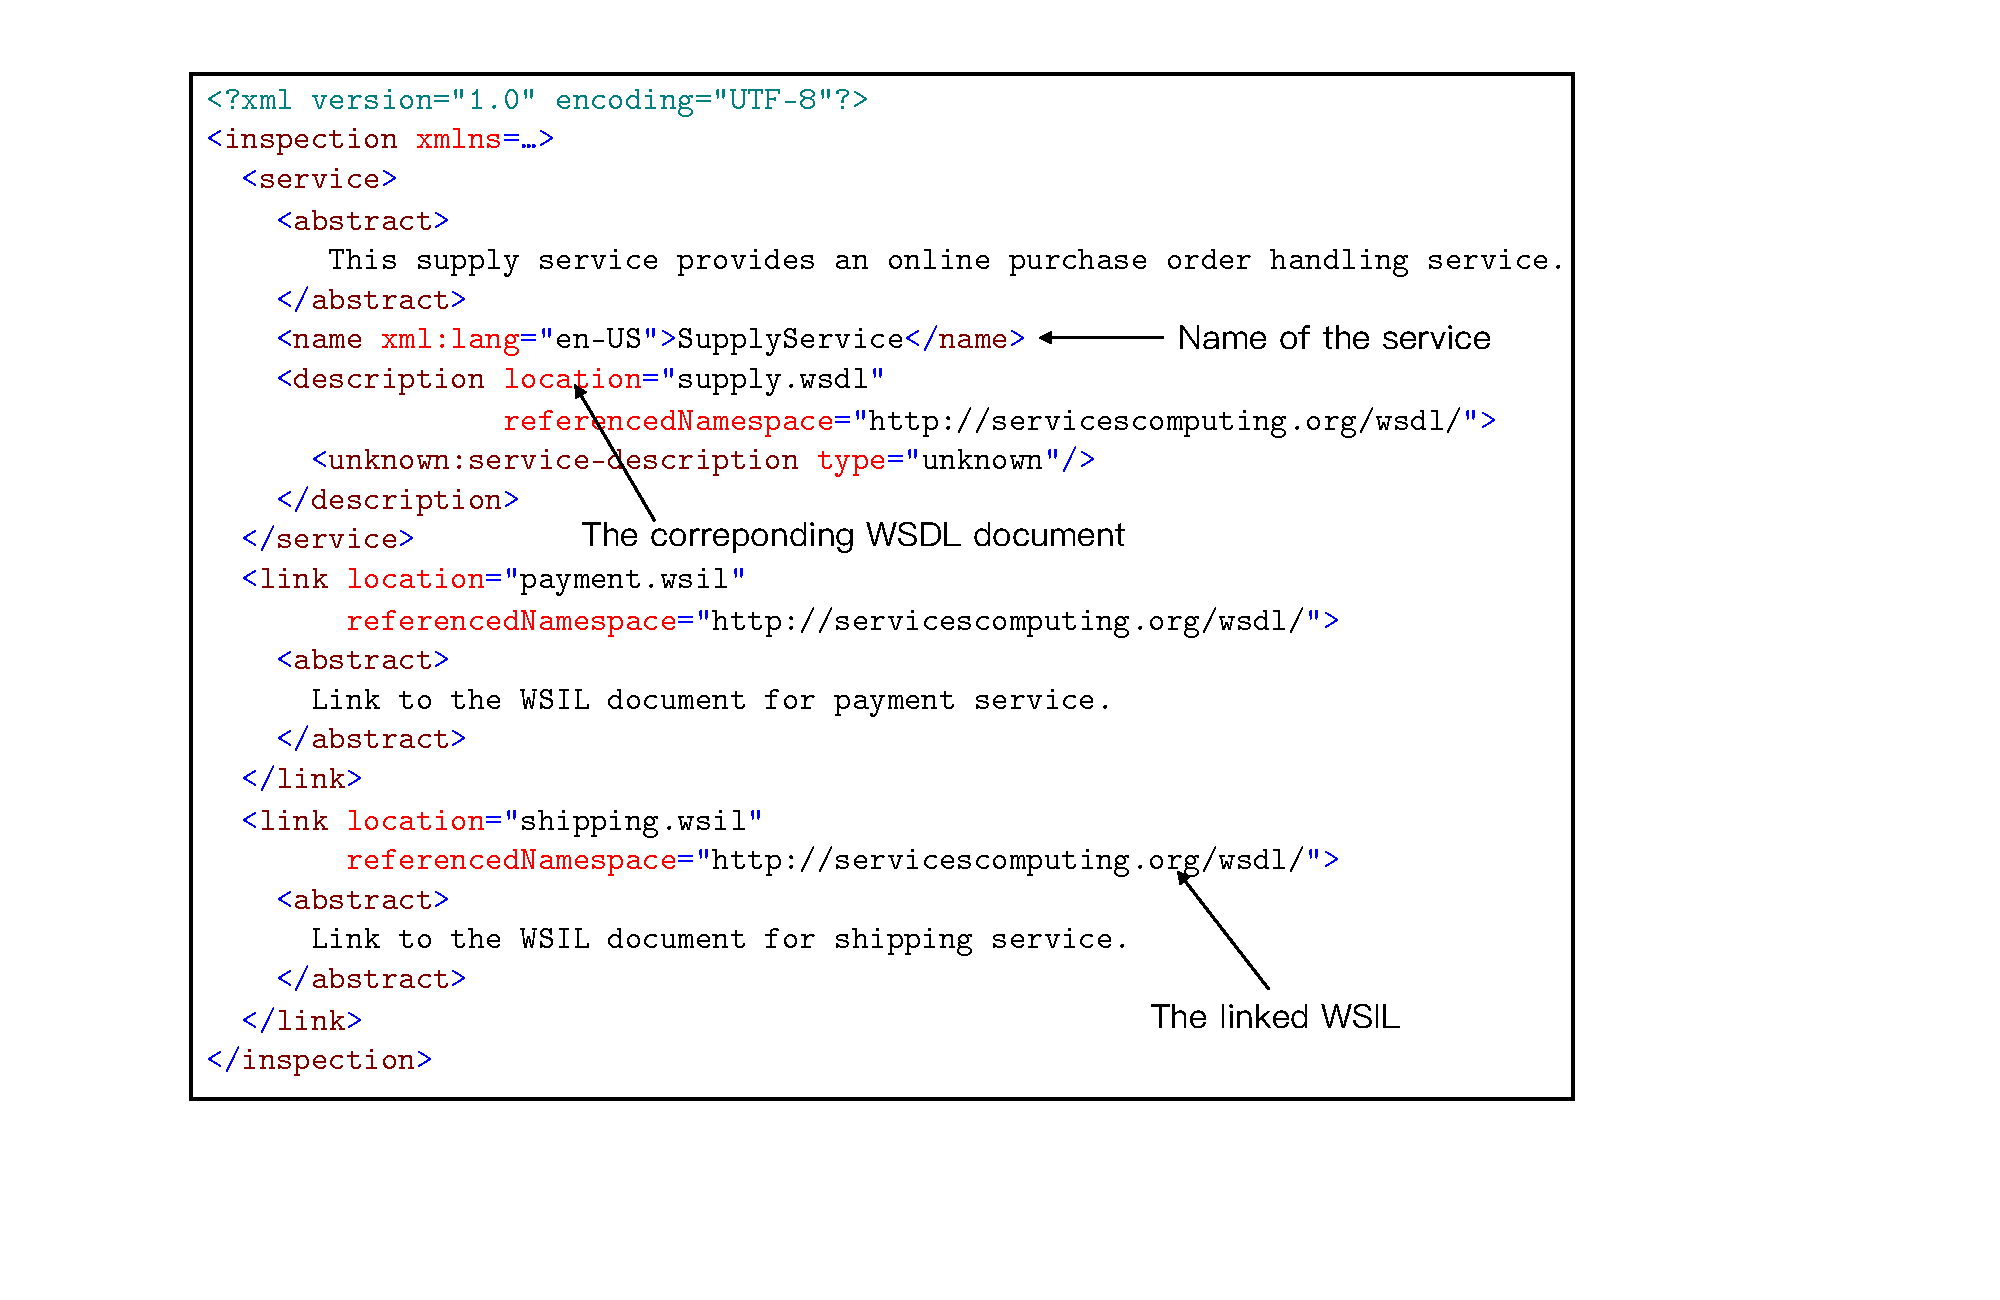
\includegraphics[width=0.75\textwidth]{images/Supply.wsil.pdf}
    \vspace{-3em}
\end{figure}

\paragraph*{Shipping.wsil}~{} \par
\begin{figure}[H]
    \vspace{-0.5em}
	\centering
	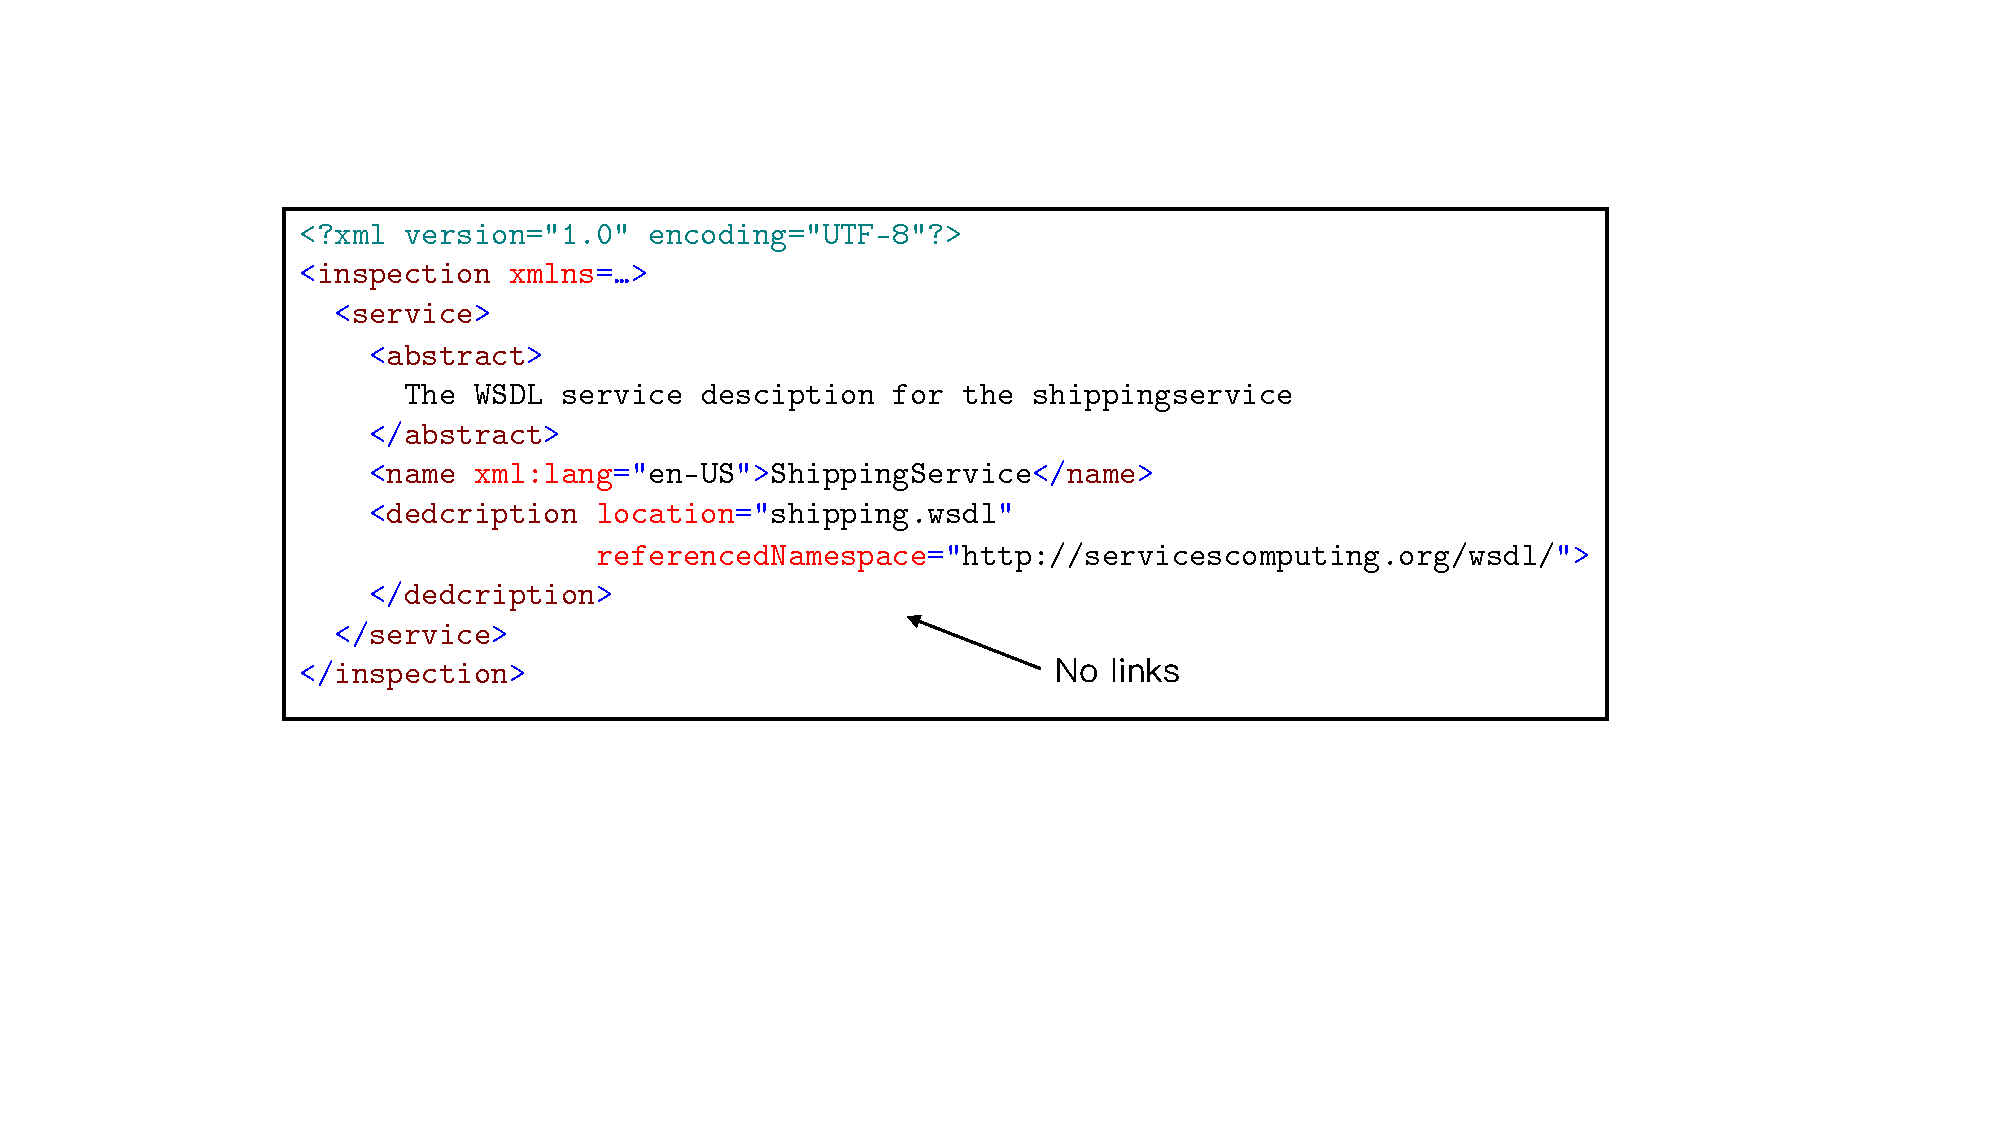
\includegraphics[width=0.75\textwidth]{images/Shipping.wsil.pdf}
    \vspace{-1em}
\end{figure}

\paragraph*{Payment.wsil}~{} \par
\begin{figure}[H]
    \vspace{-0.5em}
	\centering
	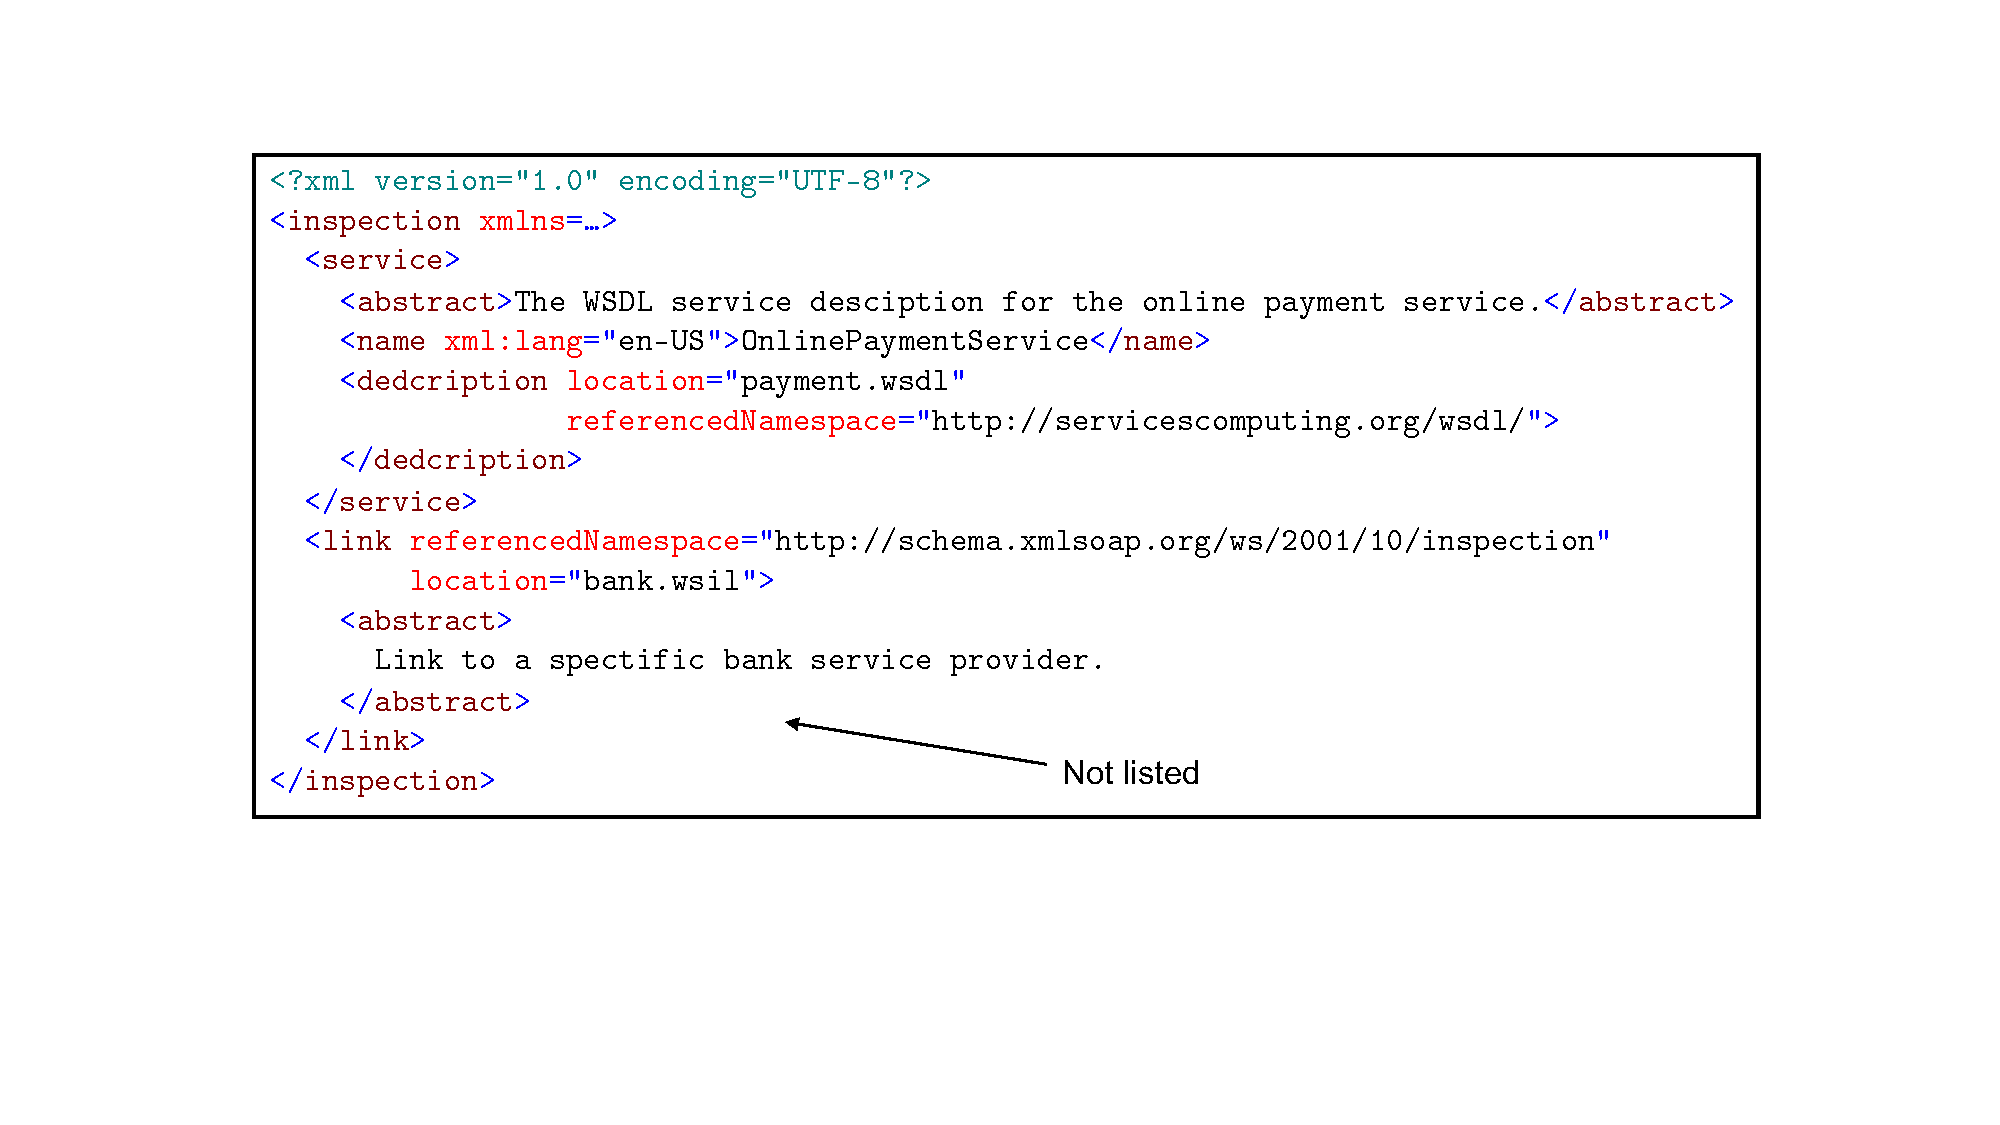
\includegraphics[width=0.85\textwidth]{images/Payment.wsil.pdf}
    \vspace{-1em}
\end{figure}

\subsubsection{UDDI发布与WSIL发布}
\begin{itemize}
    \item UDDI可以被视为传统的黄页目录,将来自各个组织的已发布Web服务进行分类和组织。
    \item WSIL使得Web服务能够通过普通Web服务器进行发现、部署和调用,而无需完整而复杂的服务注册表基础设施。
    \item 成本和复杂性是不同的,可以在黄页目录和询问信息之间进行选择。
\end{itemize}


\subsection{Web Services查询}

\begin{figure}[H]
    \vspace{-1.5em}
	\centering
	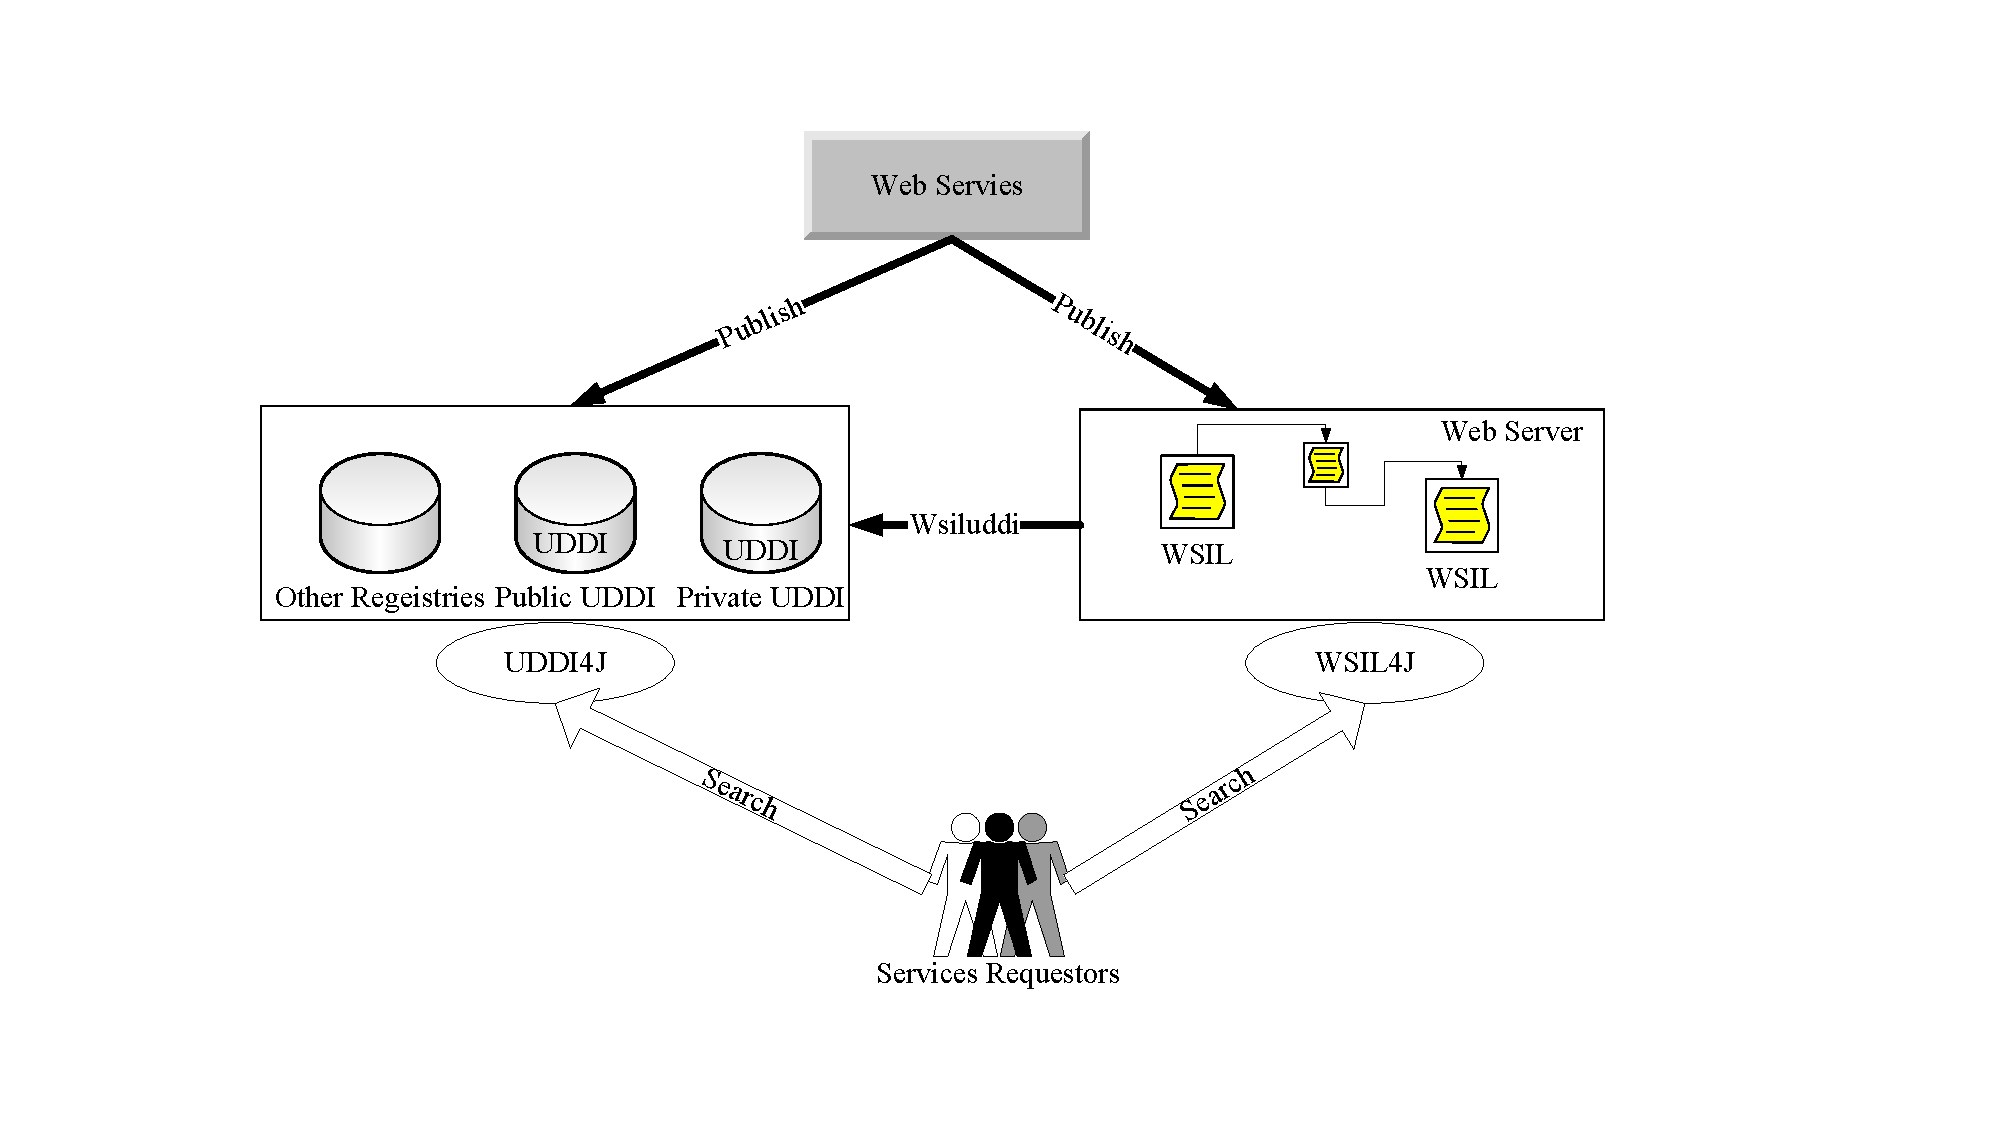
\includegraphics[width=0.7\textwidth]{images/Web Services查询.pdf}
    \vspace{-3em}
\end{figure}

\subsubsection{UDDI查询}
用UDDI客户端在UDDI注册表中查找Web服务,UDDI for Java (UDDI4J)是一个UDDI客户端例子
\begin{itemize}
    \item 它是一个Java类库,提供了与UDDI注册表进行交互的API
    \item 支持UDDI规范、SOAP传输、调试日志记录和配置功能
\end{itemize}

三种查询的方向
\begin{figure}[H]
    \vspace{-0.5em}
	\centering
	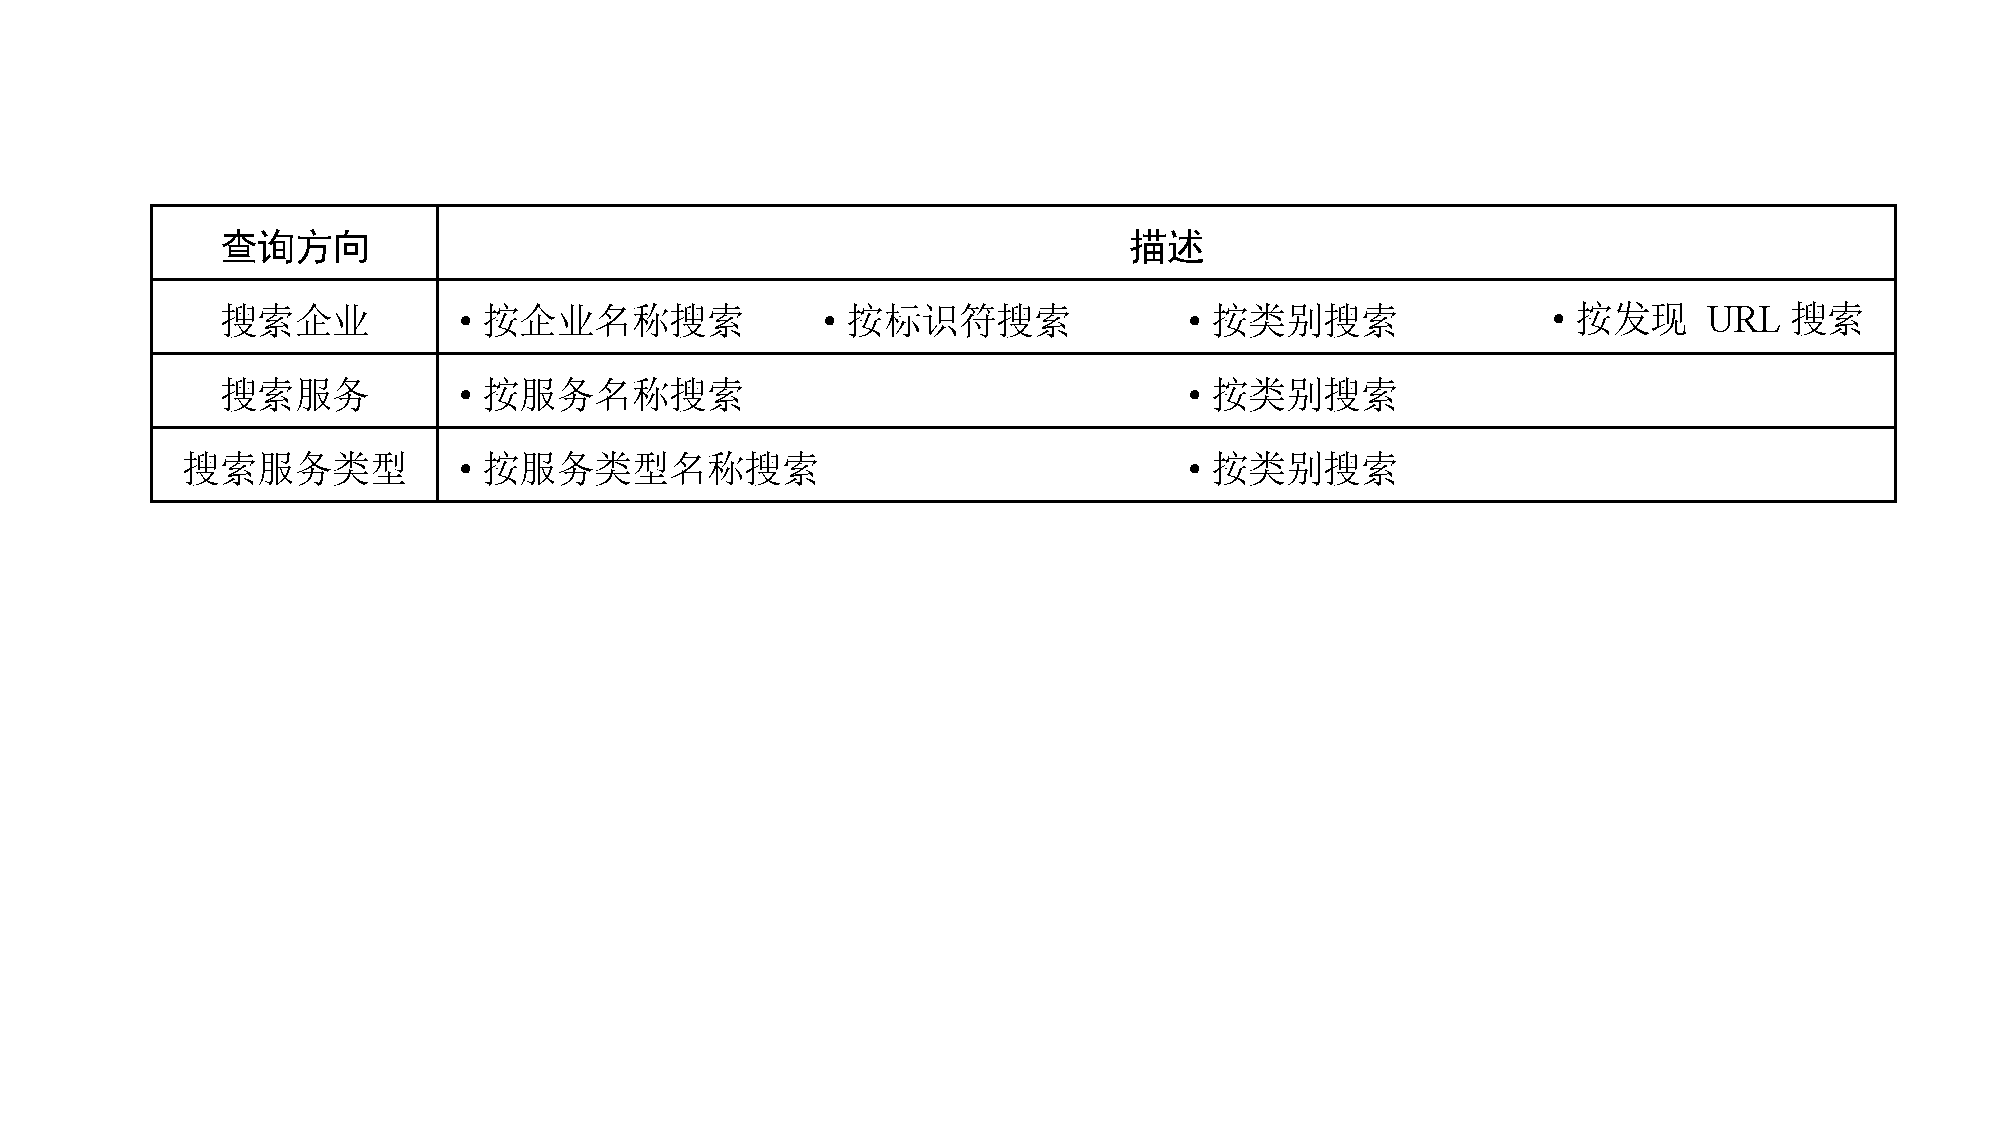
\includegraphics[width=\textwidth]{images/三种查询的方向.pdf}
    \vspace{-3em}
\end{figure}

UDDI查询API有两类使用模式
\vspace{-0.5em}
\begin{spacing}{1.2}
    \centering
    \begin{longtable}{|m{2cm}<{\centering}|m{13cm}|}
    \hline
    \textbf{使用模式} & \multicolumn{1}{c|}{\textbf{描述}} \\ \hline
    浏览 &
    \vspace{-1.3em}
    \begin{itemize}[leftmargin=1.5em,itemsep=-3pt]
        \item 开发者可以使用浏览模式(发现API调用)来获取满足比较宽泛的查询标准的接入点、服务或者技术特性
        \item 浏览模式中,可以使用\;\verb|find_business|、\verb|find_relatedBusiness|、\verb|find_service|、\verb|find_binding|\;和\;\verb|find_tModel|\;操作 
    \vspace{-1.5em}
    \end{itemize}                                           
    \\ \hline
    下钻 & 
    \vspace{-1.3em}
    \begin{itemize}[leftmargin=1.5em,itemsep=-3pt]
        \item 使用下钻模式(获取API调用)来获取更具体的功能部件
        \item 下钻模式中,可以使用\;\verb|get_businessDetail|、\verb|get_BusinessDetailExt|、\verb|get_serviceDetail|、\verb|get_bindingDetail|\;和\;\verb|get_tModelDetail|\;操作
    \vspace{-1.5em}
    \end{itemize}  
    \\ \hline
\end{longtable}
\end{spacing}
\vspace{-1em}

\subsubsection{WISL查询}
主要基于通过WSIL文档链的迭代式搜索过程:
\begin{enumerate}[label=\arabic*.]
    \item 确定起始WSIL文档的位置
    \item 执行指定的WSIL文档搜索
    \item 显示包含在WSIL文档中的链接列表
    \item 选择链接以启动所选WSIL文档的内容。如果所启动的文档包含其他链接,请追踪链接以检索进一步的文档
    \item 重复步骤3和4,迭代所有相关的链接,直到找到所需信息
\end{enumerate}

通常通过构建在WSIL解析器之上的搜索工具执行。例如,Web服务检查语言的Java API (WSIL4J),用于解析现有的WSIL文档或以编程方式创建新的WSIL文档。
\vspace{-0.8em}
\begin{multicols}{2}
    \begin{itemize}
        \item 提供WSIL元素的类
        \item 包括WSILProxy,以访问WSIL文档中的信息
    \end{itemize}
\end{multicols}
\vspace{-1em}

\subsubsection{JAXR}
JAXR是一种标准的Java API,用于在不同类型的注册表上执行注册操作。它提供了描述业务注册表内容的统一信息模型,并提供了多层API抽象,是JavaEE平台中Web服务的关键技术之一。

JAXR不是新的注册表标准,它定义了用于访问各种当前和未来注册表的Java API,同时它也不是最小公共分母API\footnote{最小公共分母API (Least Common Denominator API)指的是一种API设计原则,旨在提供一组最基本的接口,以使不同的系统能够相互操作。这种API通常具有最小的功能集,并采用最基本的数据格式和协议,以确保能够在尽可能多的系统上运行。但是,这种API可能会受到限制,无法支持某些高级特性或自定义扩展。},JAXR支持主流注册表规范中最好的特性的结合。

\begin{wraptable}{r}{8.6cm}
    \centering
    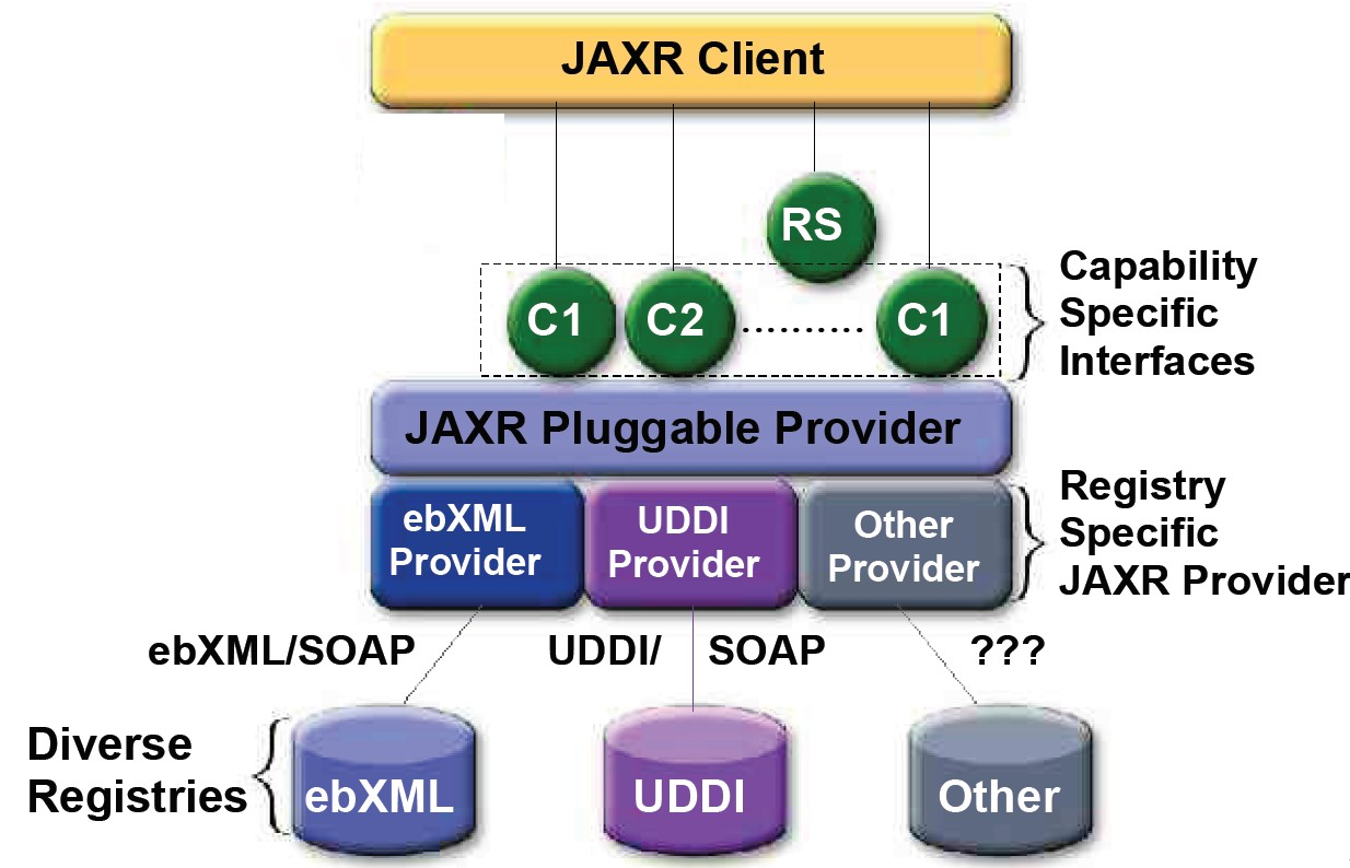
\includegraphics[width=8.5cm]{images/JAXR.png}
    \vspace{-5.5em}
\end{wraptable}
注册表提供程序(Registry Provider)
\begin{itemize}
    \item 提供注册表规范的实现
    \item 不需要实现JAXR规范
    \item 例如:UDDI注册表,ebXML注册表
\end{itemize}

JAXR提供程序(JAXR Provider)
\begin{itemize}
    \item 实现JAXR规范
    \item 通常作为现有注册表提供程序的门面功能
    \item 例如:JAXR参考实现
\end{itemize}

JAXR客户端(JAXR Client)
\begin{itemize}
    \item 使用JAXR API来访问JAXR提供程序提供的服务
\end{itemize}
